\documentclass{article}
\usepackage{nott-titlepage}
\usepackage{graphicx}
\usepackage{pdfpages}
\usepackage{biblatex}
\usepackage{float}
\usepackage{siunitx}
\usepackage{circuitikz}
\usepackage{tikz}
\usetikzlibrary{calc}

\title{Amplifier Design Report}
\author{Tan Hong Kai}
\date{May 1, 2024}
\studentid{20386501}
\module{EEEE3117 Analogue Electronics}
\department{Department of Electrical and Electronics Engineering}

\addbibresource{main.bib}

\begin{document}
\maketitle

\section{Introduction}

This coursework explores the design of a mid-band multistage amplifier.
The amplifier consists of 3 transistors.
The first two stages is a BJT and the third is a MOSFET.
Figure \ref{fig:amp-circuit} shows the configuration of the amplifier circuit while, table \ref{tab:component-parameters} shows the parameters given.
The resistor values consists of digits from the student ID: “20386501”.
The resistor values should be chosen such that the gain of the amplifier is between 50 and 400.
Furthermore, the transistor must be operating in the correct region.

\begin{table}[H]
    \caption{Component Parameters Given for the Design}
    \label{tab:component-parameters}
    \centering
    \begin{tabular}{ l l }
        \hline
        Parameter & Value         \\
        \hline
        $V_{CC}$  & $15 V$        \\
        $R_{S}$   & $8 k\Omega$   \\
        $R_{L}$   & $300 \Omega$  \\
        $V_{BE}$  & $0.7 V$       \\
        $\beta$   & $150$         \\
        $V_{A}$   & $65 V$        \\
        $K_{n}$   & $5 mA/V^{2}$  \\
        $V_{TN}$  & $-2 V$        \\
        $\lambda$ & $0.01 V^{-1}$ \\
        $C$       & $22 \mu{F}$   \\
        \hline
    \end{tabular}
\end{table}

\begin{figure}[H]
    \centering
    \resizebox{\textwidth}{!}{
        \begin{circuitikz}[american]
            % Input Voltage
            \draw (0, 0) to[resistor, R=$R_{S}$] (2, 0) to[capacitor, -*] (4, 0);
            \draw (0, 0) to [vsource, V=$V_{s}$] (0, -3) to (4, -3);

            % Q1
            \draw (6, 0) node[npn](Q1){Q1};
            \draw (4, 0) to (Q1.B);
            \draw (Q1.E) to[resistor, R=$R_{E1}$, -*] (6, -3) to (4, -3);
            \draw (6, 3) to[resistor, R=$R_{C1}$] (Q1.C);
            \draw (6, 3) to[short, *-] (4, 3) to[resistor, R=$R_{11}$] (4, 0) to[resistor, R=$R_{21}$, -*] (4, -3);
            \draw (Q1.E) to[short, *-] ++(2, 0) to [capacitor, -*] (8, -3) to (6, -3);
            \draw (Q1.C) to[capacitor] ++(2, 0) to (8, 0) to[short, -*] ++(1, 0);

            % Q2
            \draw (11, 0) node[npn](Q2){Q2};
            \draw (9, 0) to (Q2.B);
            \draw (Q2.E) to[resistor, R=$R_{E2}$, -*] (11, -3) to ++(-3, 0);
            \draw (11, 3) to[resistor, R=$R_{C2}$] (Q2.C);
            \draw (6, 3) to[short, -*] (9, 3) to[resistor, R=$R_{12}$] ++(0, -3) to[resistor, R=$R_{22}$, -*] ++(0, -3);
            \draw (9, 3) to[short, -*] ++(2, 0);
            \draw (Q2.E) to[short, *-] ++(2, 0) to [capacitor, -*] (13, -3) to ++(-2, 0);
            \draw (Q2.C) to[capacitor] ++(2, 0) to (13, 0) to[short, -*] ++(1, 0) node[anchor=east](M3_start){};

            % M3
            \draw (M3_start) ++(2, 0) node[nmos](M3){M3};
            \draw (M3_start) to (M3.G);
            \draw (11, 3) to[short, -*] ++(3, 0) to[resistor, R=$R_{13}$] ++(0, -3) to[resistor, R=$R_{23}$, -*] ++(0, -3) to ++(-1, 0);
            \draw (M3.D) to[short, -o] ++(0, 2.23) node[anchor=west]{$V_{CC}$} to ++(-2, 0);
            % https://tex.stackexchange.com/questions/18389/tikz-node-at-same-x-coordinate-as-another-node-but-specified-y-coordinate
            \draw (M3.S) to[resistor, R=$R_{SS}$, *-*] (M3.S |-, -3) to ++(2, 0) node[anchor=north](R_L){};
            \draw (M3.S) to[capacitor] ++(2, 0) to[resistor, R=$R_{L}$] (R_L);
            \draw (M3.S |-, -3) to ++(-2, 0);

            % Vo
            \draw (M3.S) ++(2, 0) to[short, -o] ++(0.5, 0) node[anchor=west]{$v_o$};
            % Ground
            \draw (Q2.E |-, -3) to (Q2.E |-, -3.1) node[ground]{};
        \end{circuitikz}
    }
    \caption{Amplifier Circuit}
    \label{fig:amp-circuit}
\end{figure}

\section{Transistor configurations}

Table \ref{tab:transistor-config} shows the transistor configurations.
From the configuration, the amplifier would have a moderate to high gain, large input impedance and small output impedance.

\begin{table}[H]
    \caption{Transistor Configurations}
    \label{tab:transistor-config}
    \centering
    \begin{tabular}{ l l }
        \hline
        Transistor & Configuration  \\
        \hline
        Q1         & Common Emitter \\
        Q2         & Common Emitter \\
        M3         & Common Drain   \\
        \hline
    \end{tabular}
\end{table}

\section{Small-Signal Equivalent Circuit}

\begin{figure}[H]
    \centering
    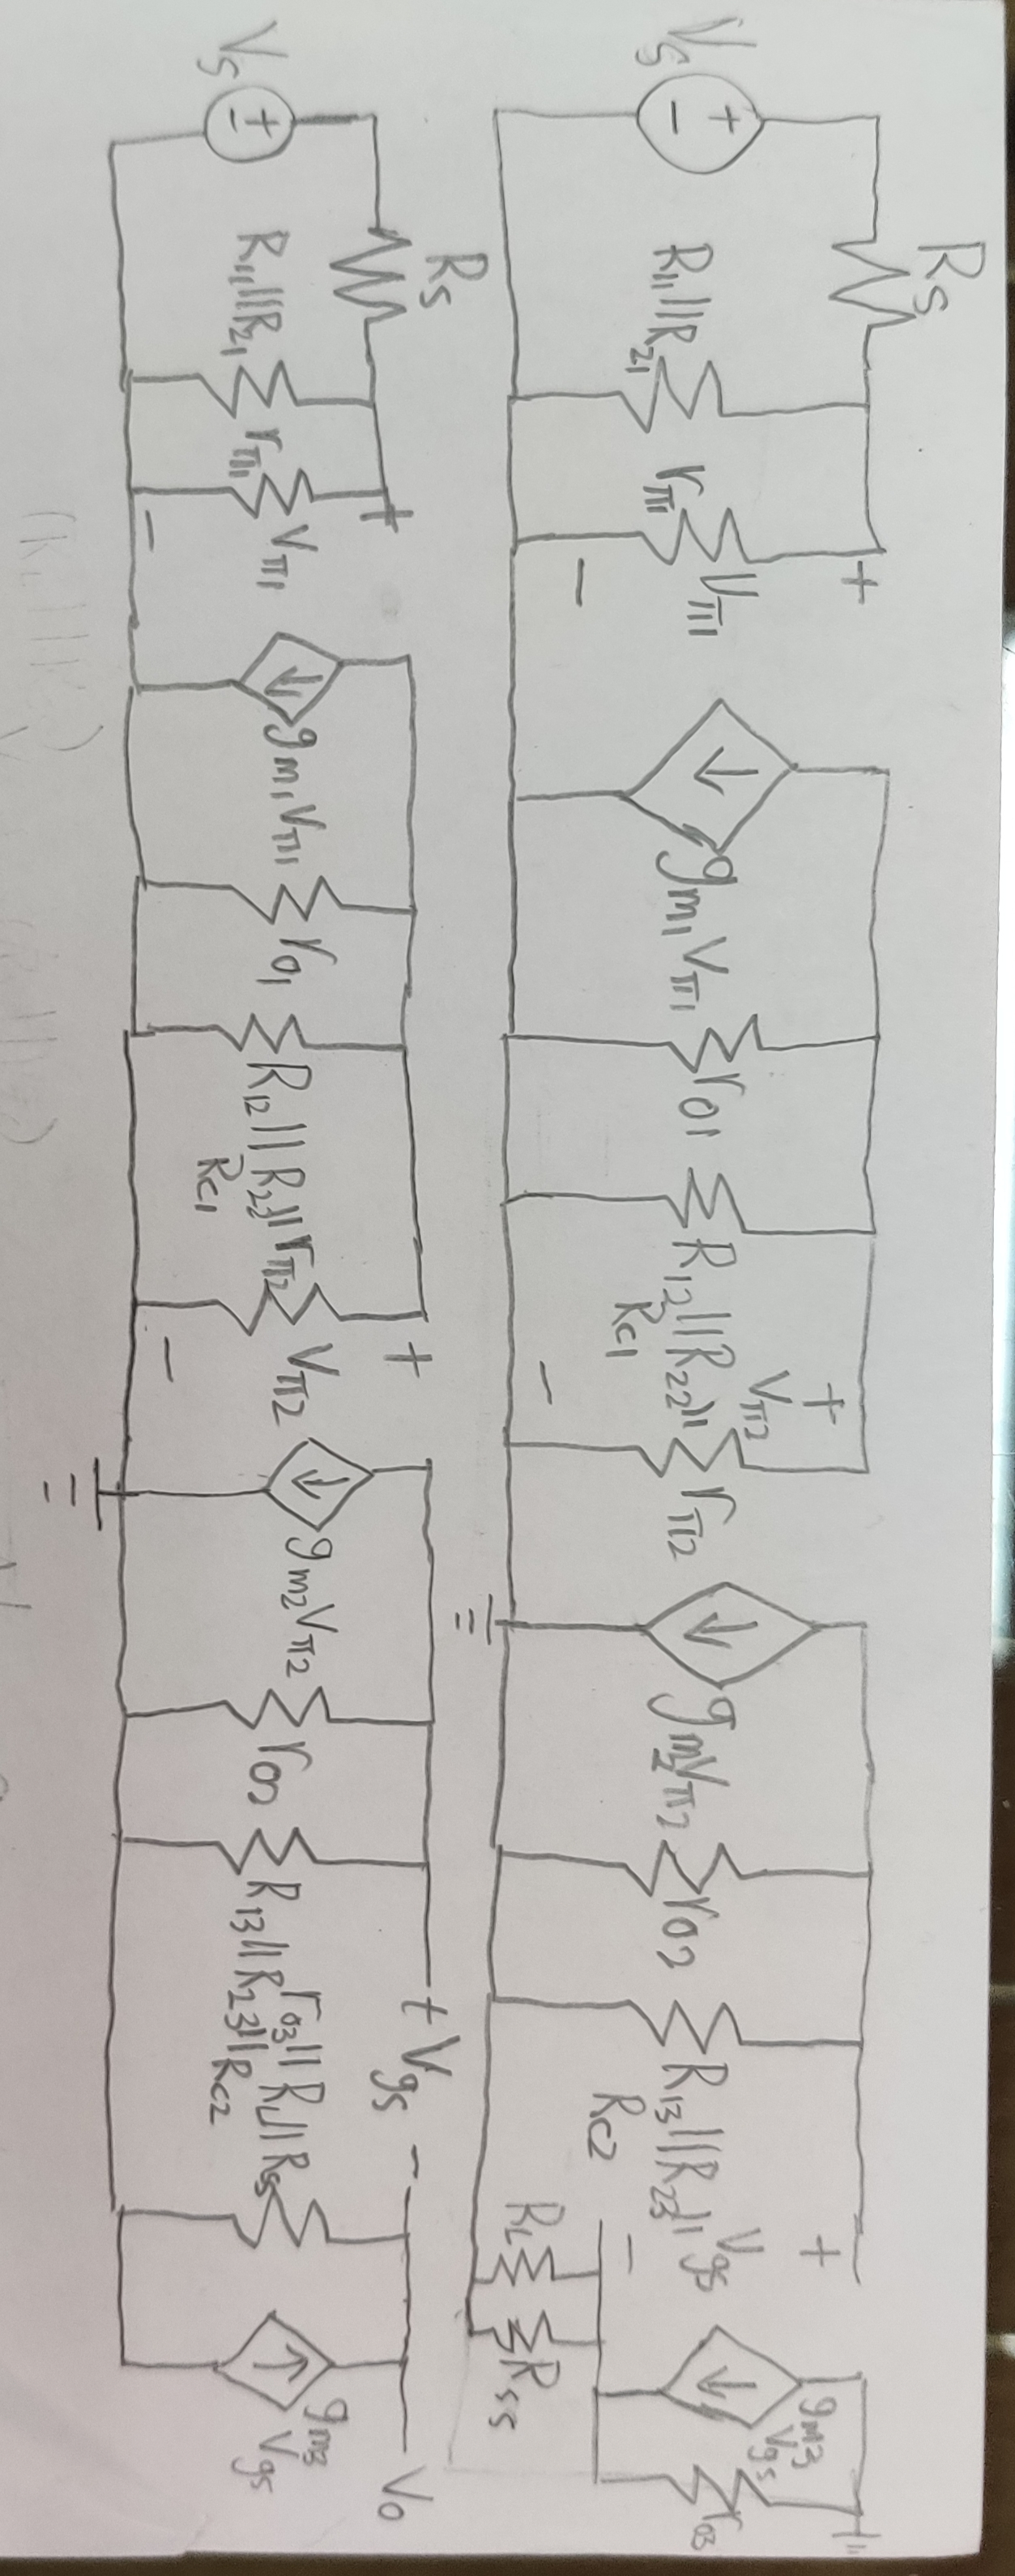
\includegraphics[height=\linewidth, angle=90]{img/small-signal-equivalent.jpeg}
    \caption{Mid-Band Small-Signal Equivalent Circuit}
    \label{fig:ss-eq-circuit}
\end{figure}

\section{Amplifier Design}

A Python script is created to help the iteration of different resistor values.
Formulas of the values are calculated by hand first, then transferred into functions in the script.
Table \ref{tab:resistor-values} shows the resistor values calculated that fits the design requirements.

\begin{table}[H]
    \caption{Resistor Values Used for Amplifier Design}
    \label{tab:resistor-values}
    \centering
    \begin{tabular}{l l l}
        \hline
        Resistor & Value ($\Omega$) & Student ID \\
        \hline
        $R_{11}$ & $1 k\Omega$      & 1          \\
        $R_{21}$ & $501 \Omega$     & 501        \\
        $R_{C1}$ & $1 k\Omega$      & 1          \\
        $R_{E1}$ & $500 \Omega$     & 5          \\
        \hline
        $R_{12}$ & $6 k\Omega$      & 6          \\
        $R_{22}$ & $8 k\Omega$      & 8          \\
        $R_{C2}$ & $2 k\Omega$      & 2          \\
        $R_{E2}$ & $3.8 k\Omega$    & 38         \\
        \hline
        $R_{13}$ & $1 k\Omega$      & 1          \\
        $R_{23}$ & $6.5 k\Omega$    & 65         \\
        $R_{SS}$ & $80 k\Omega$     & 8          \\
        \hline
    \end{tabular}
\end{table}

Using the resistor value chosen, the amplifier gain is 67.537.
This is well within the design requirements of 50 to 400.

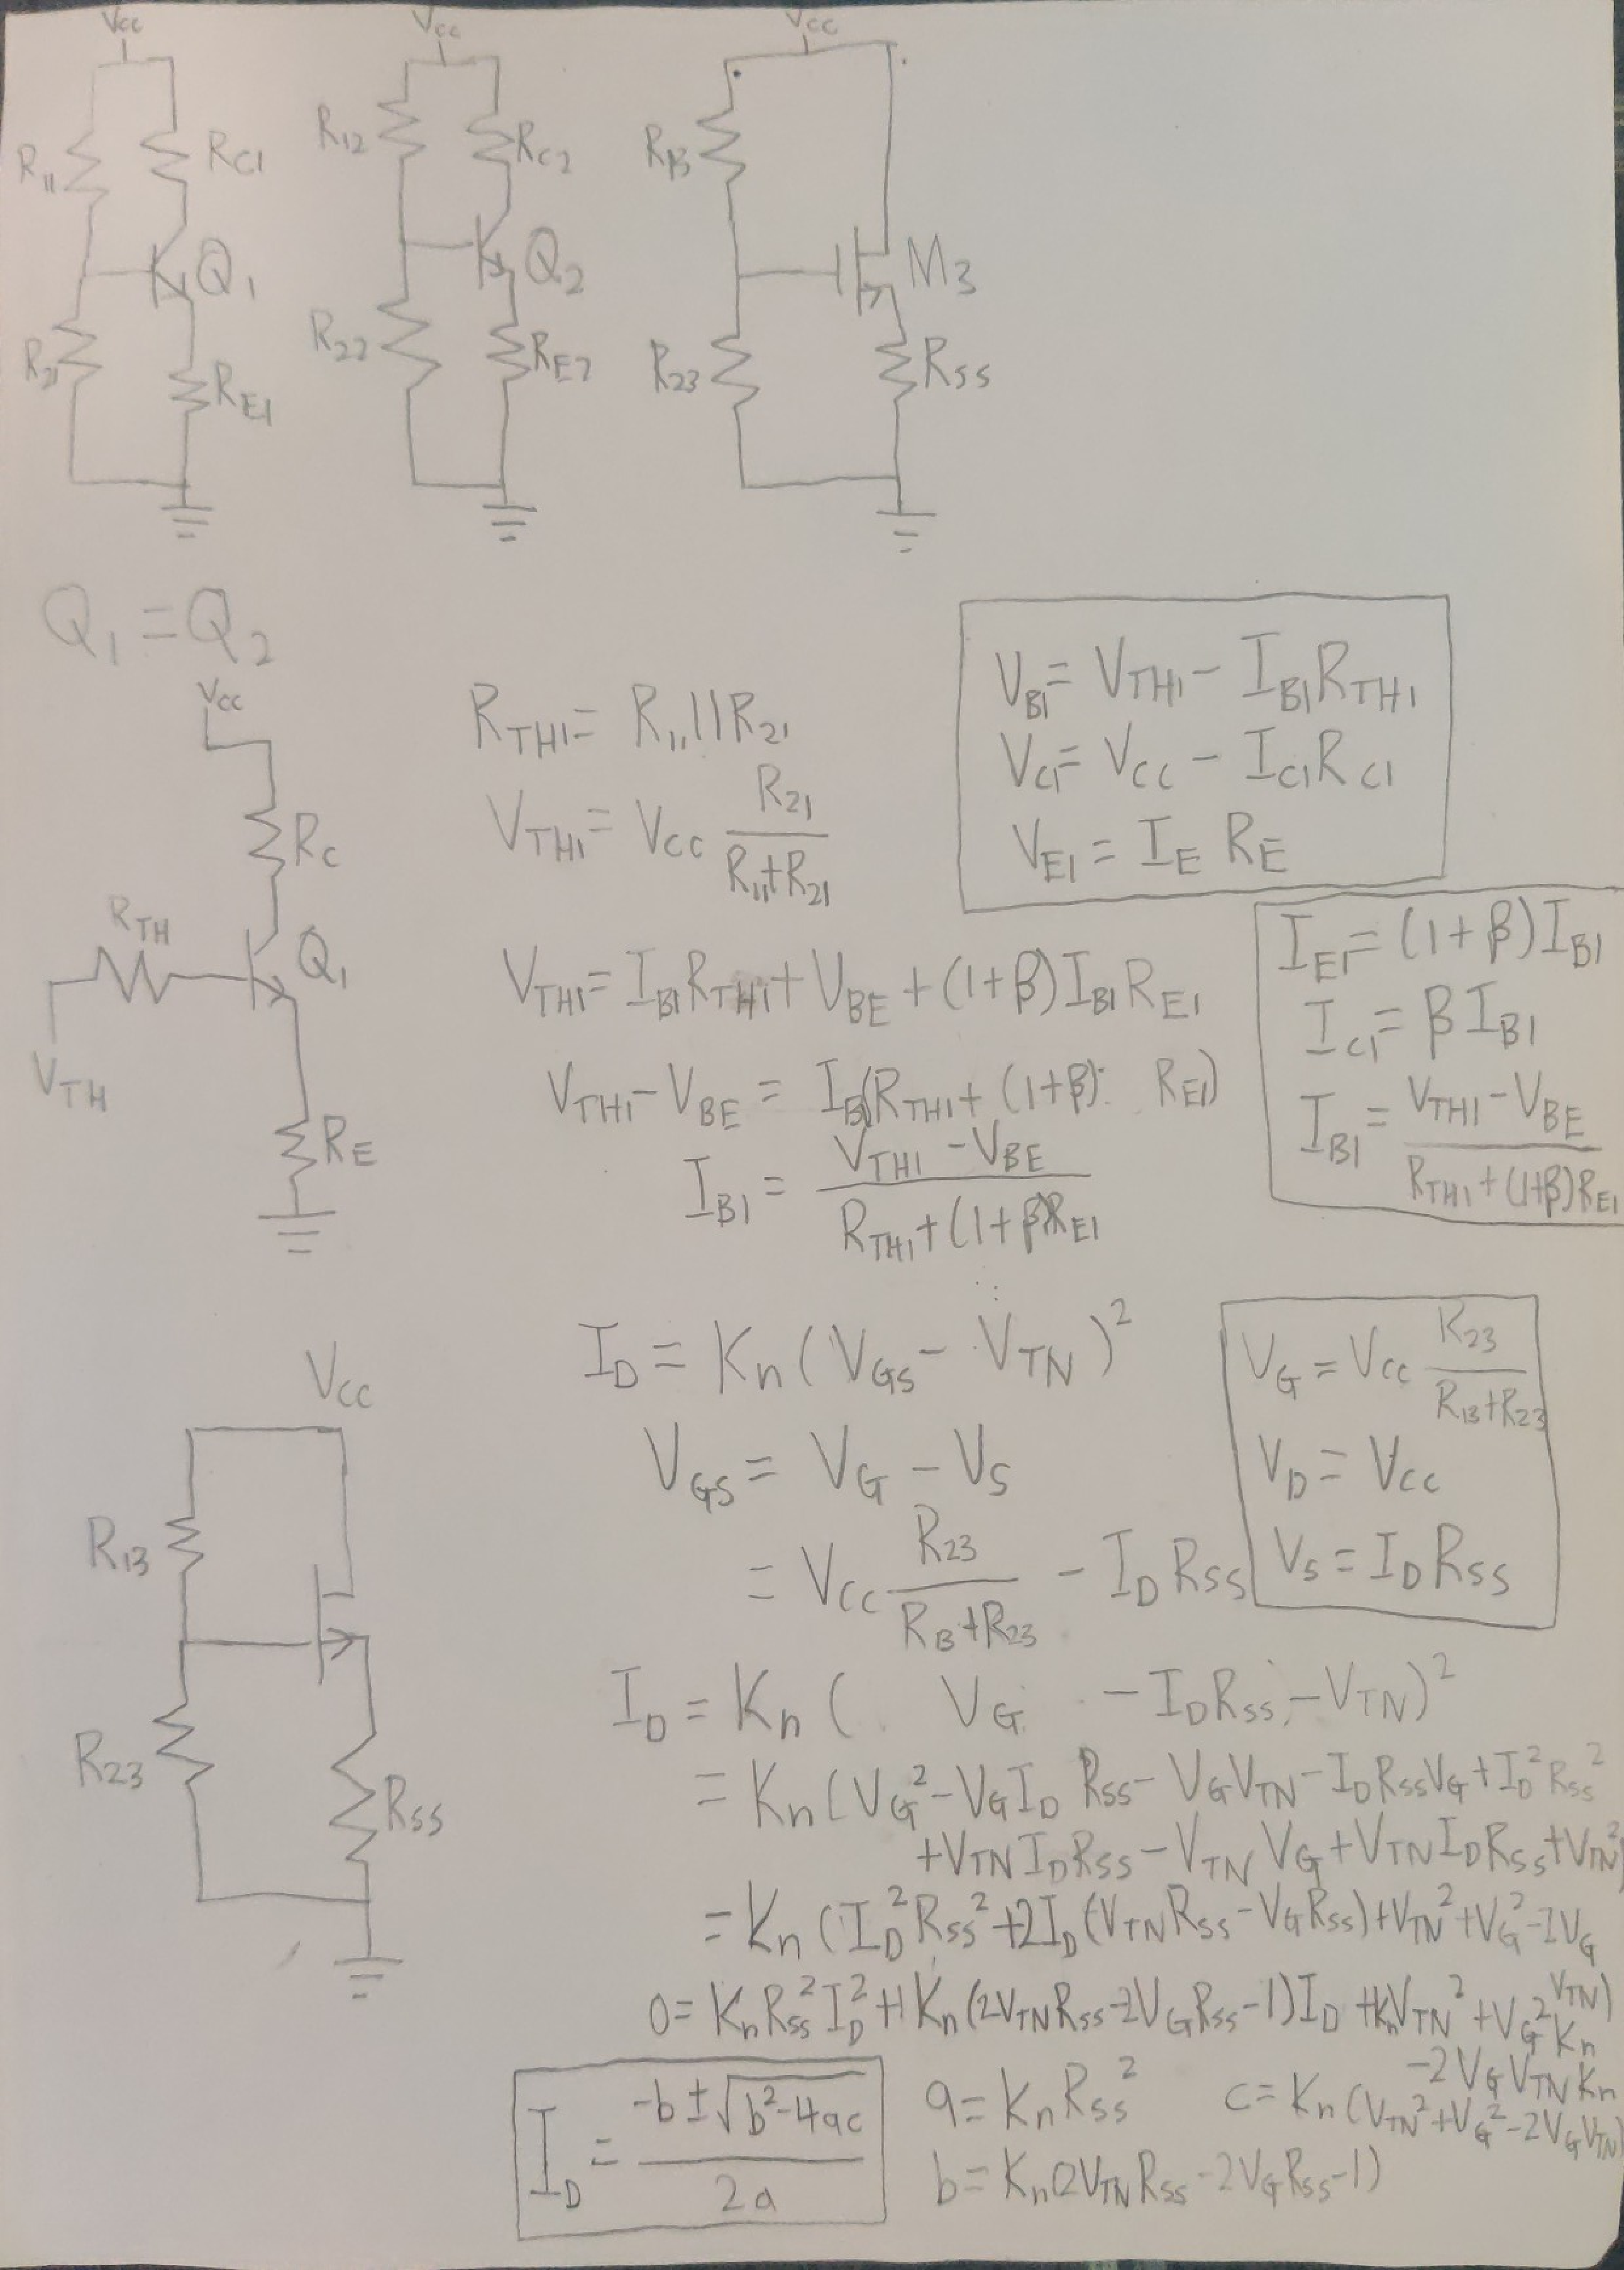
\includepdf[pages=1]{img/dc-analysis.pdf}
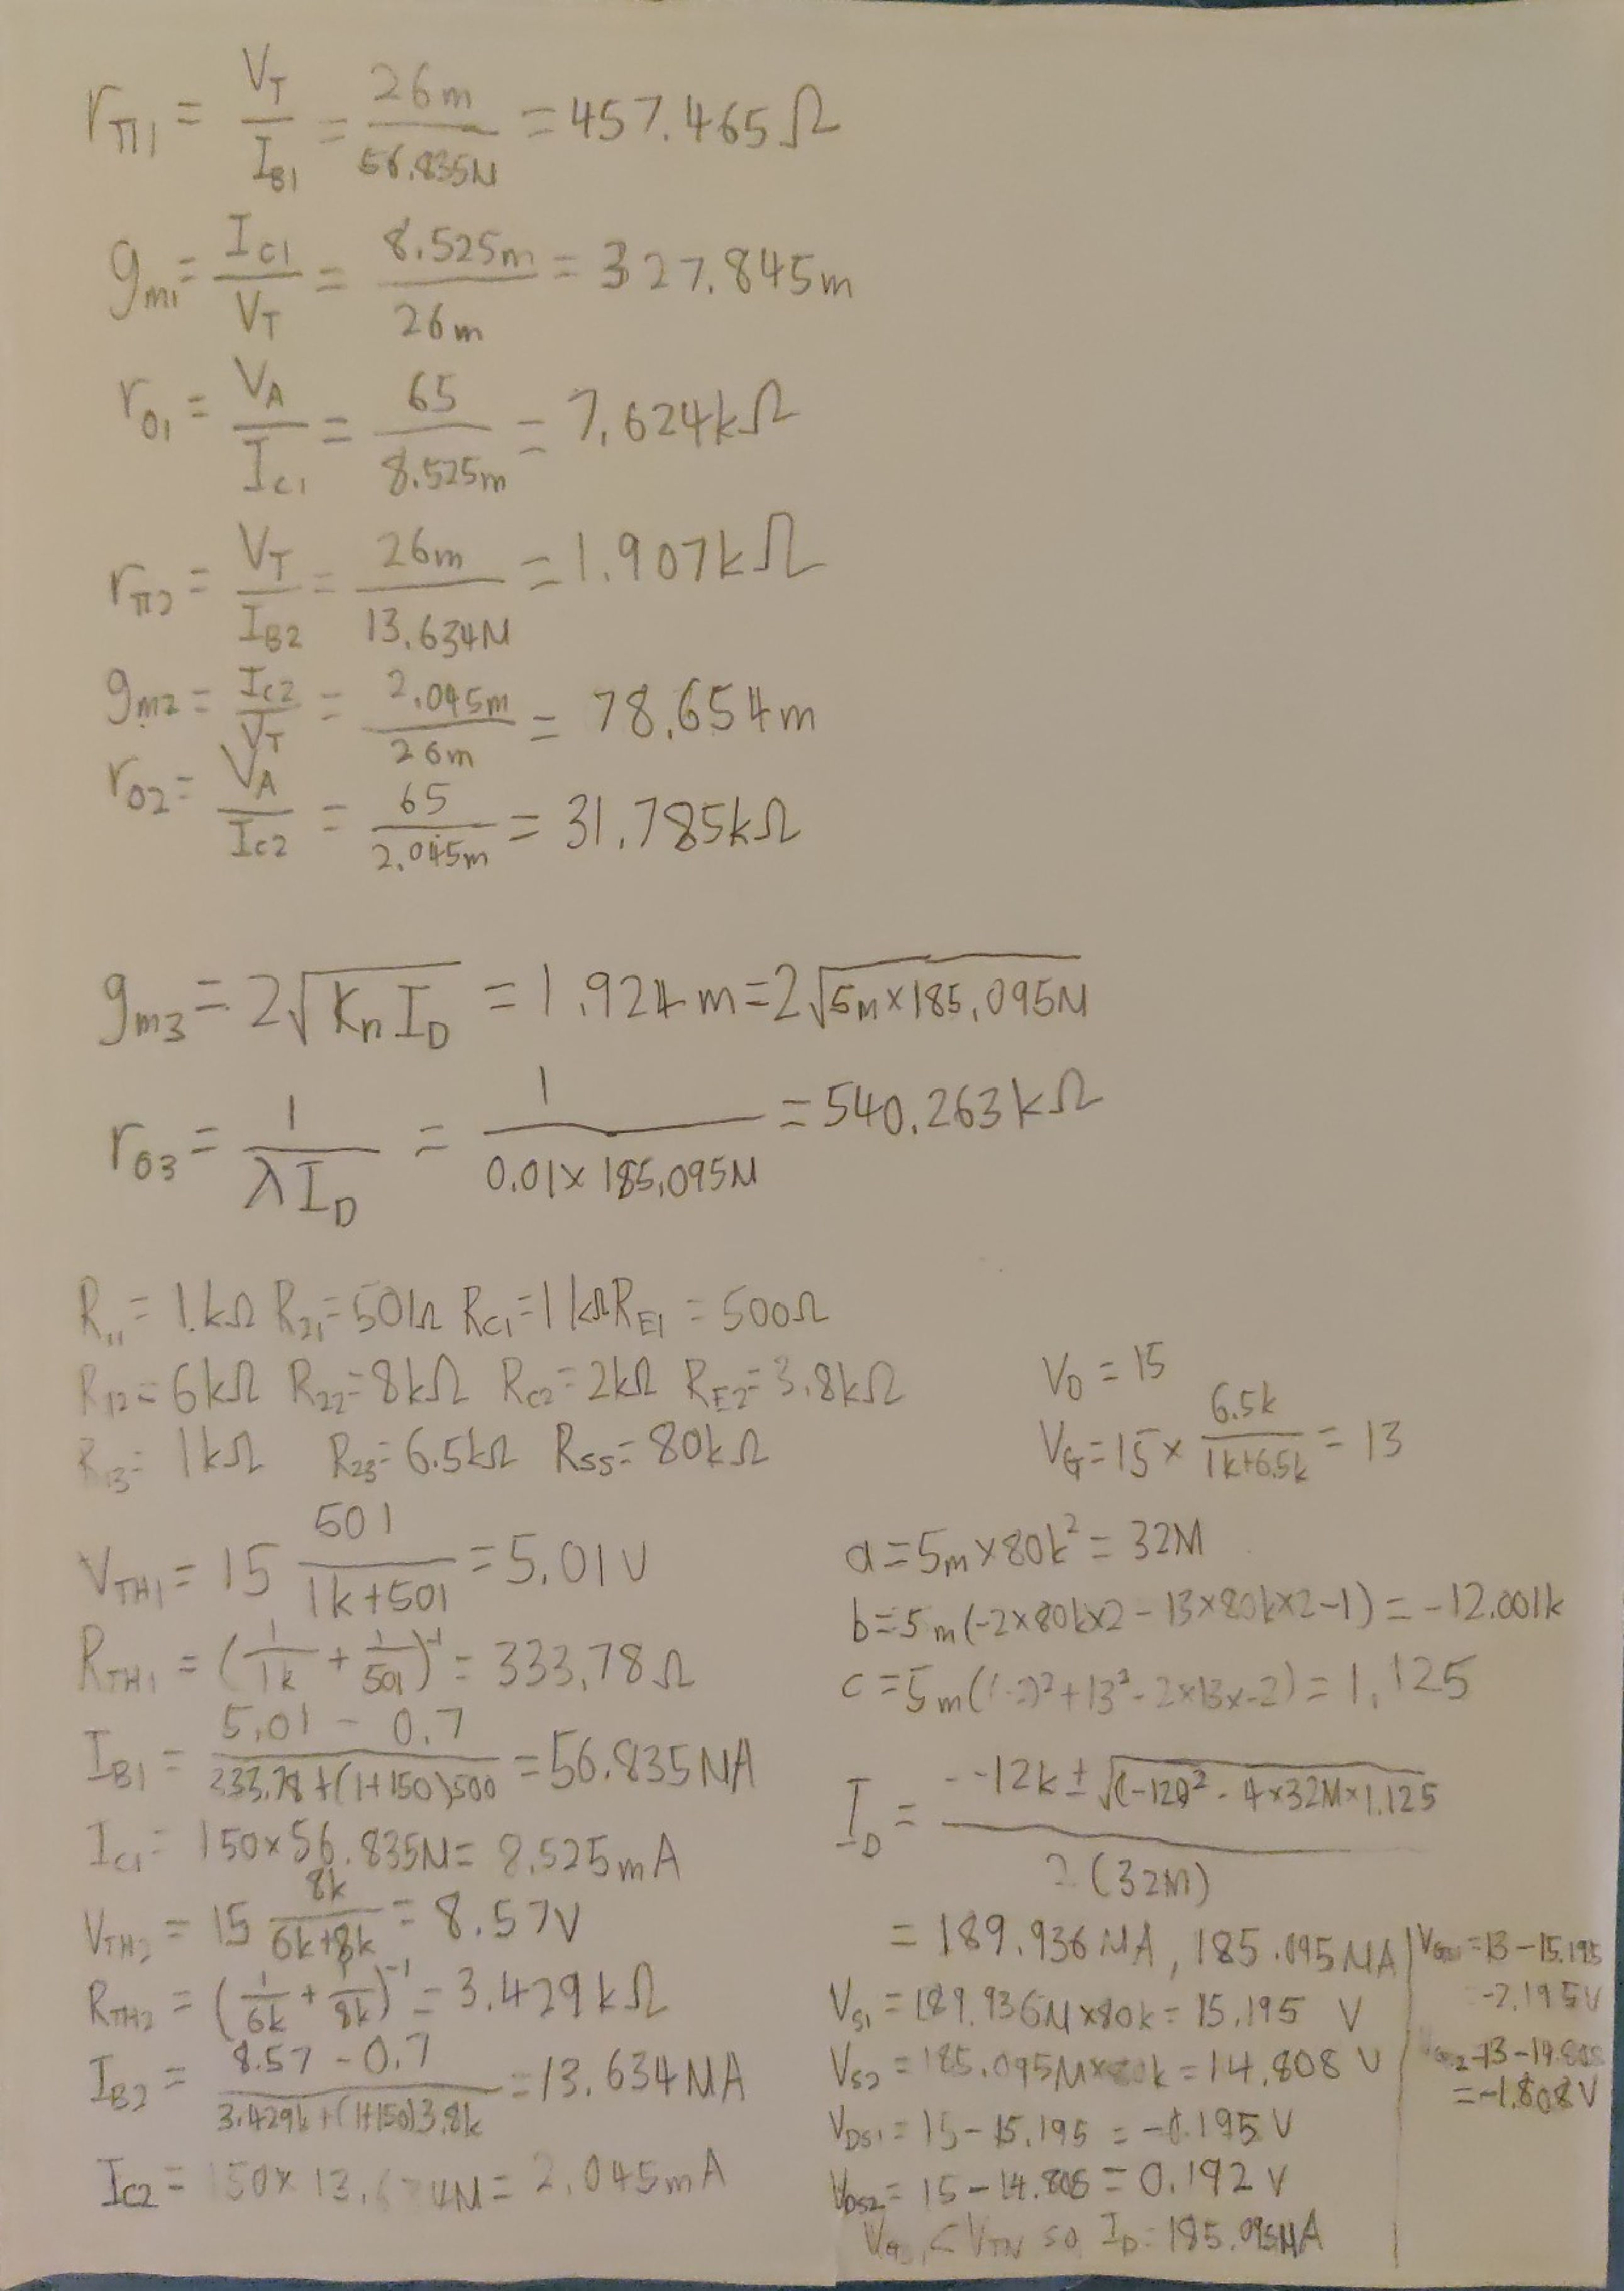
\includepdf[pages=1]{img/dc-analysis-2.pdf}
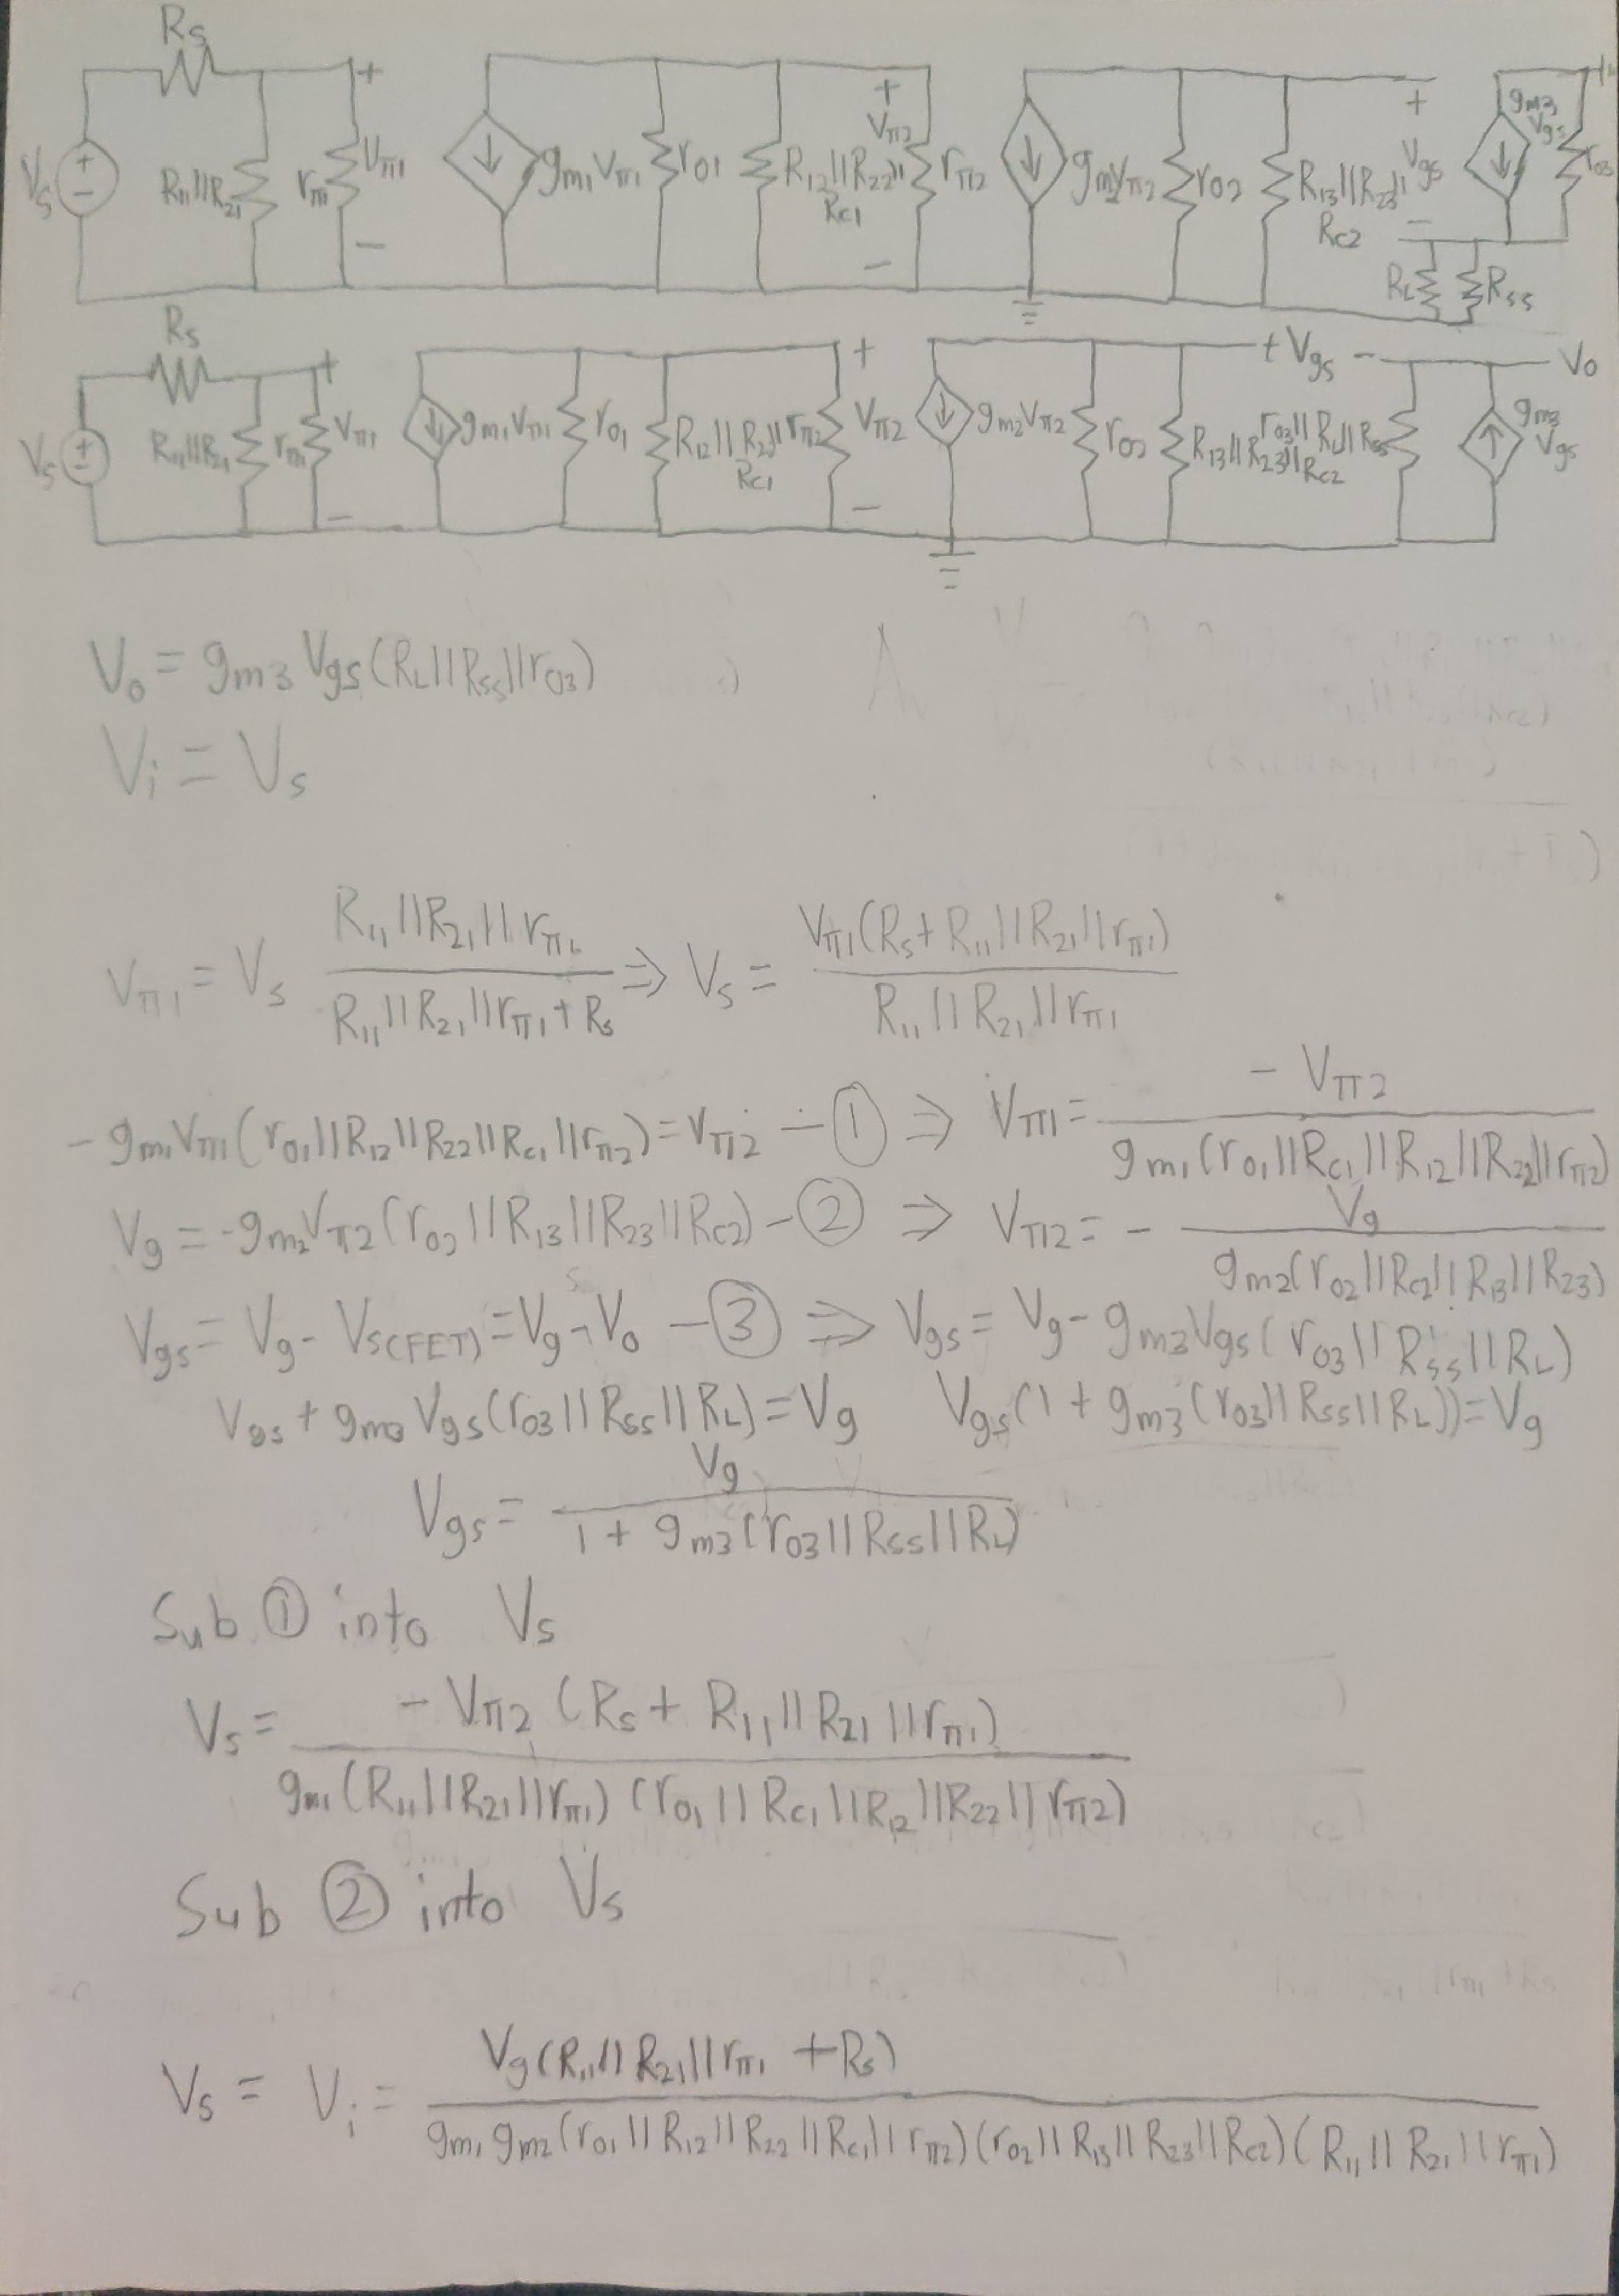
\includepdf[pages=1-]{img/ac-gain.pdf}
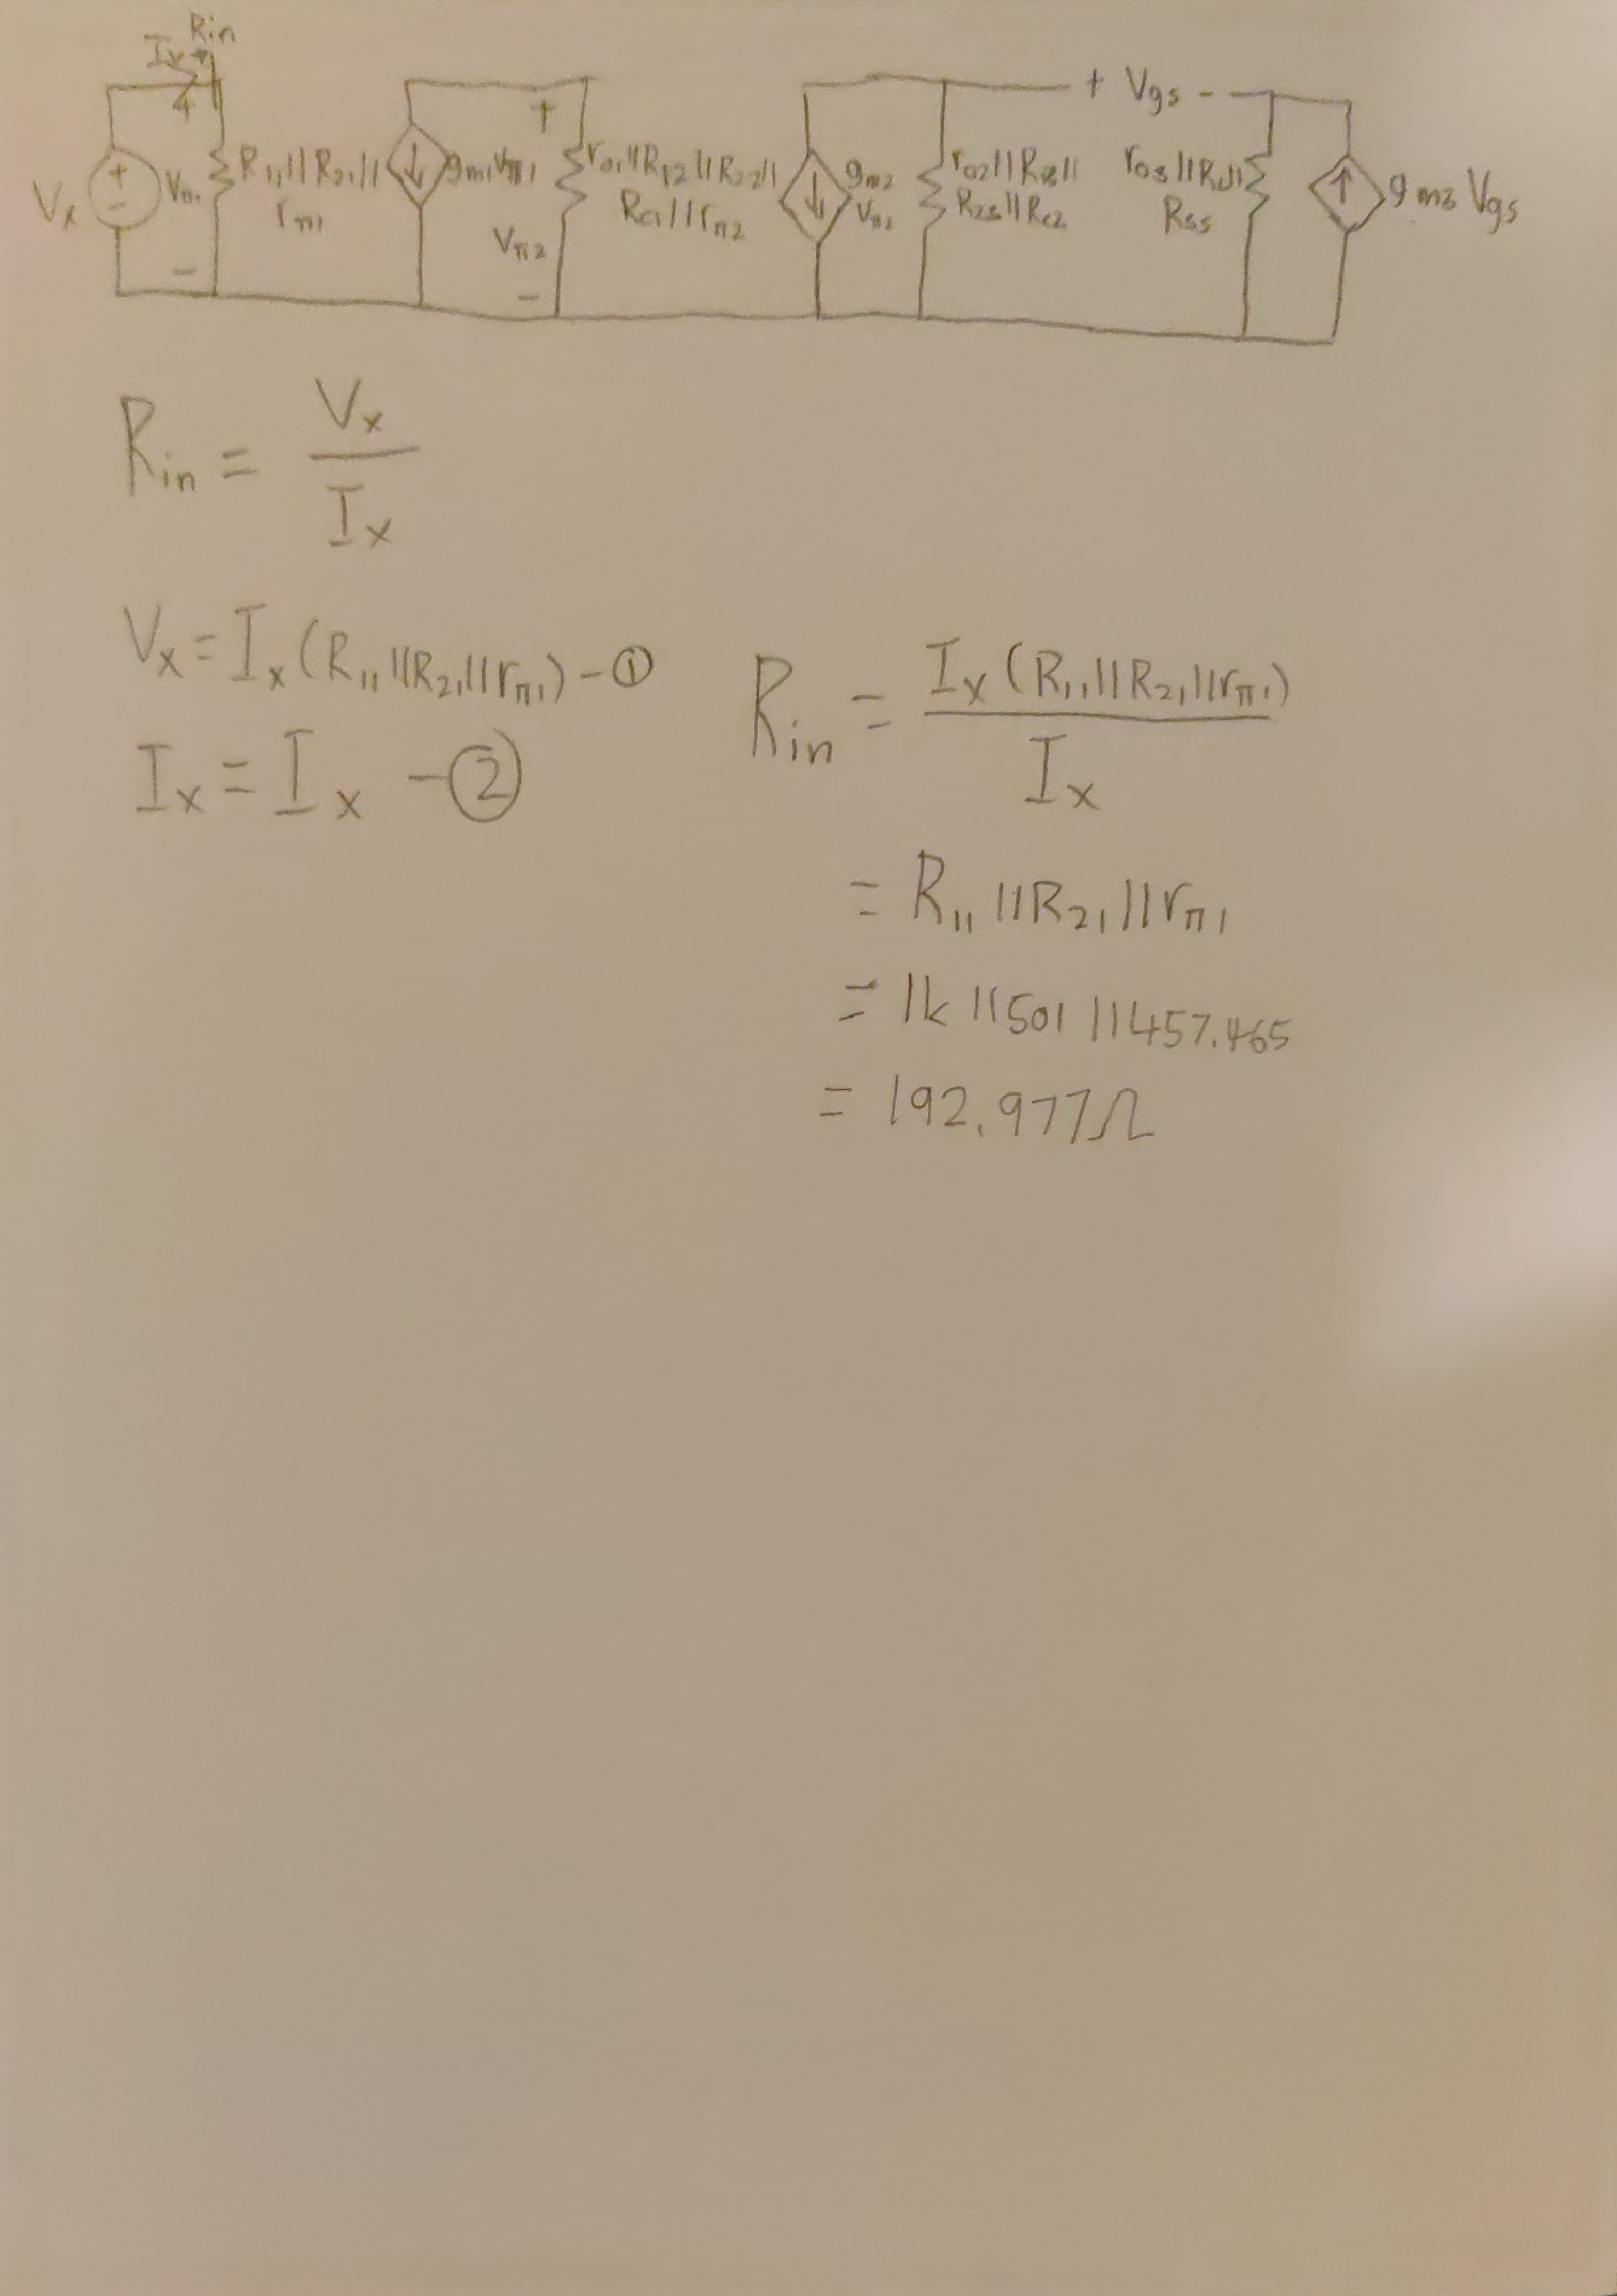
\includepdf[pages=1-]{img/input-resistance.pdf}
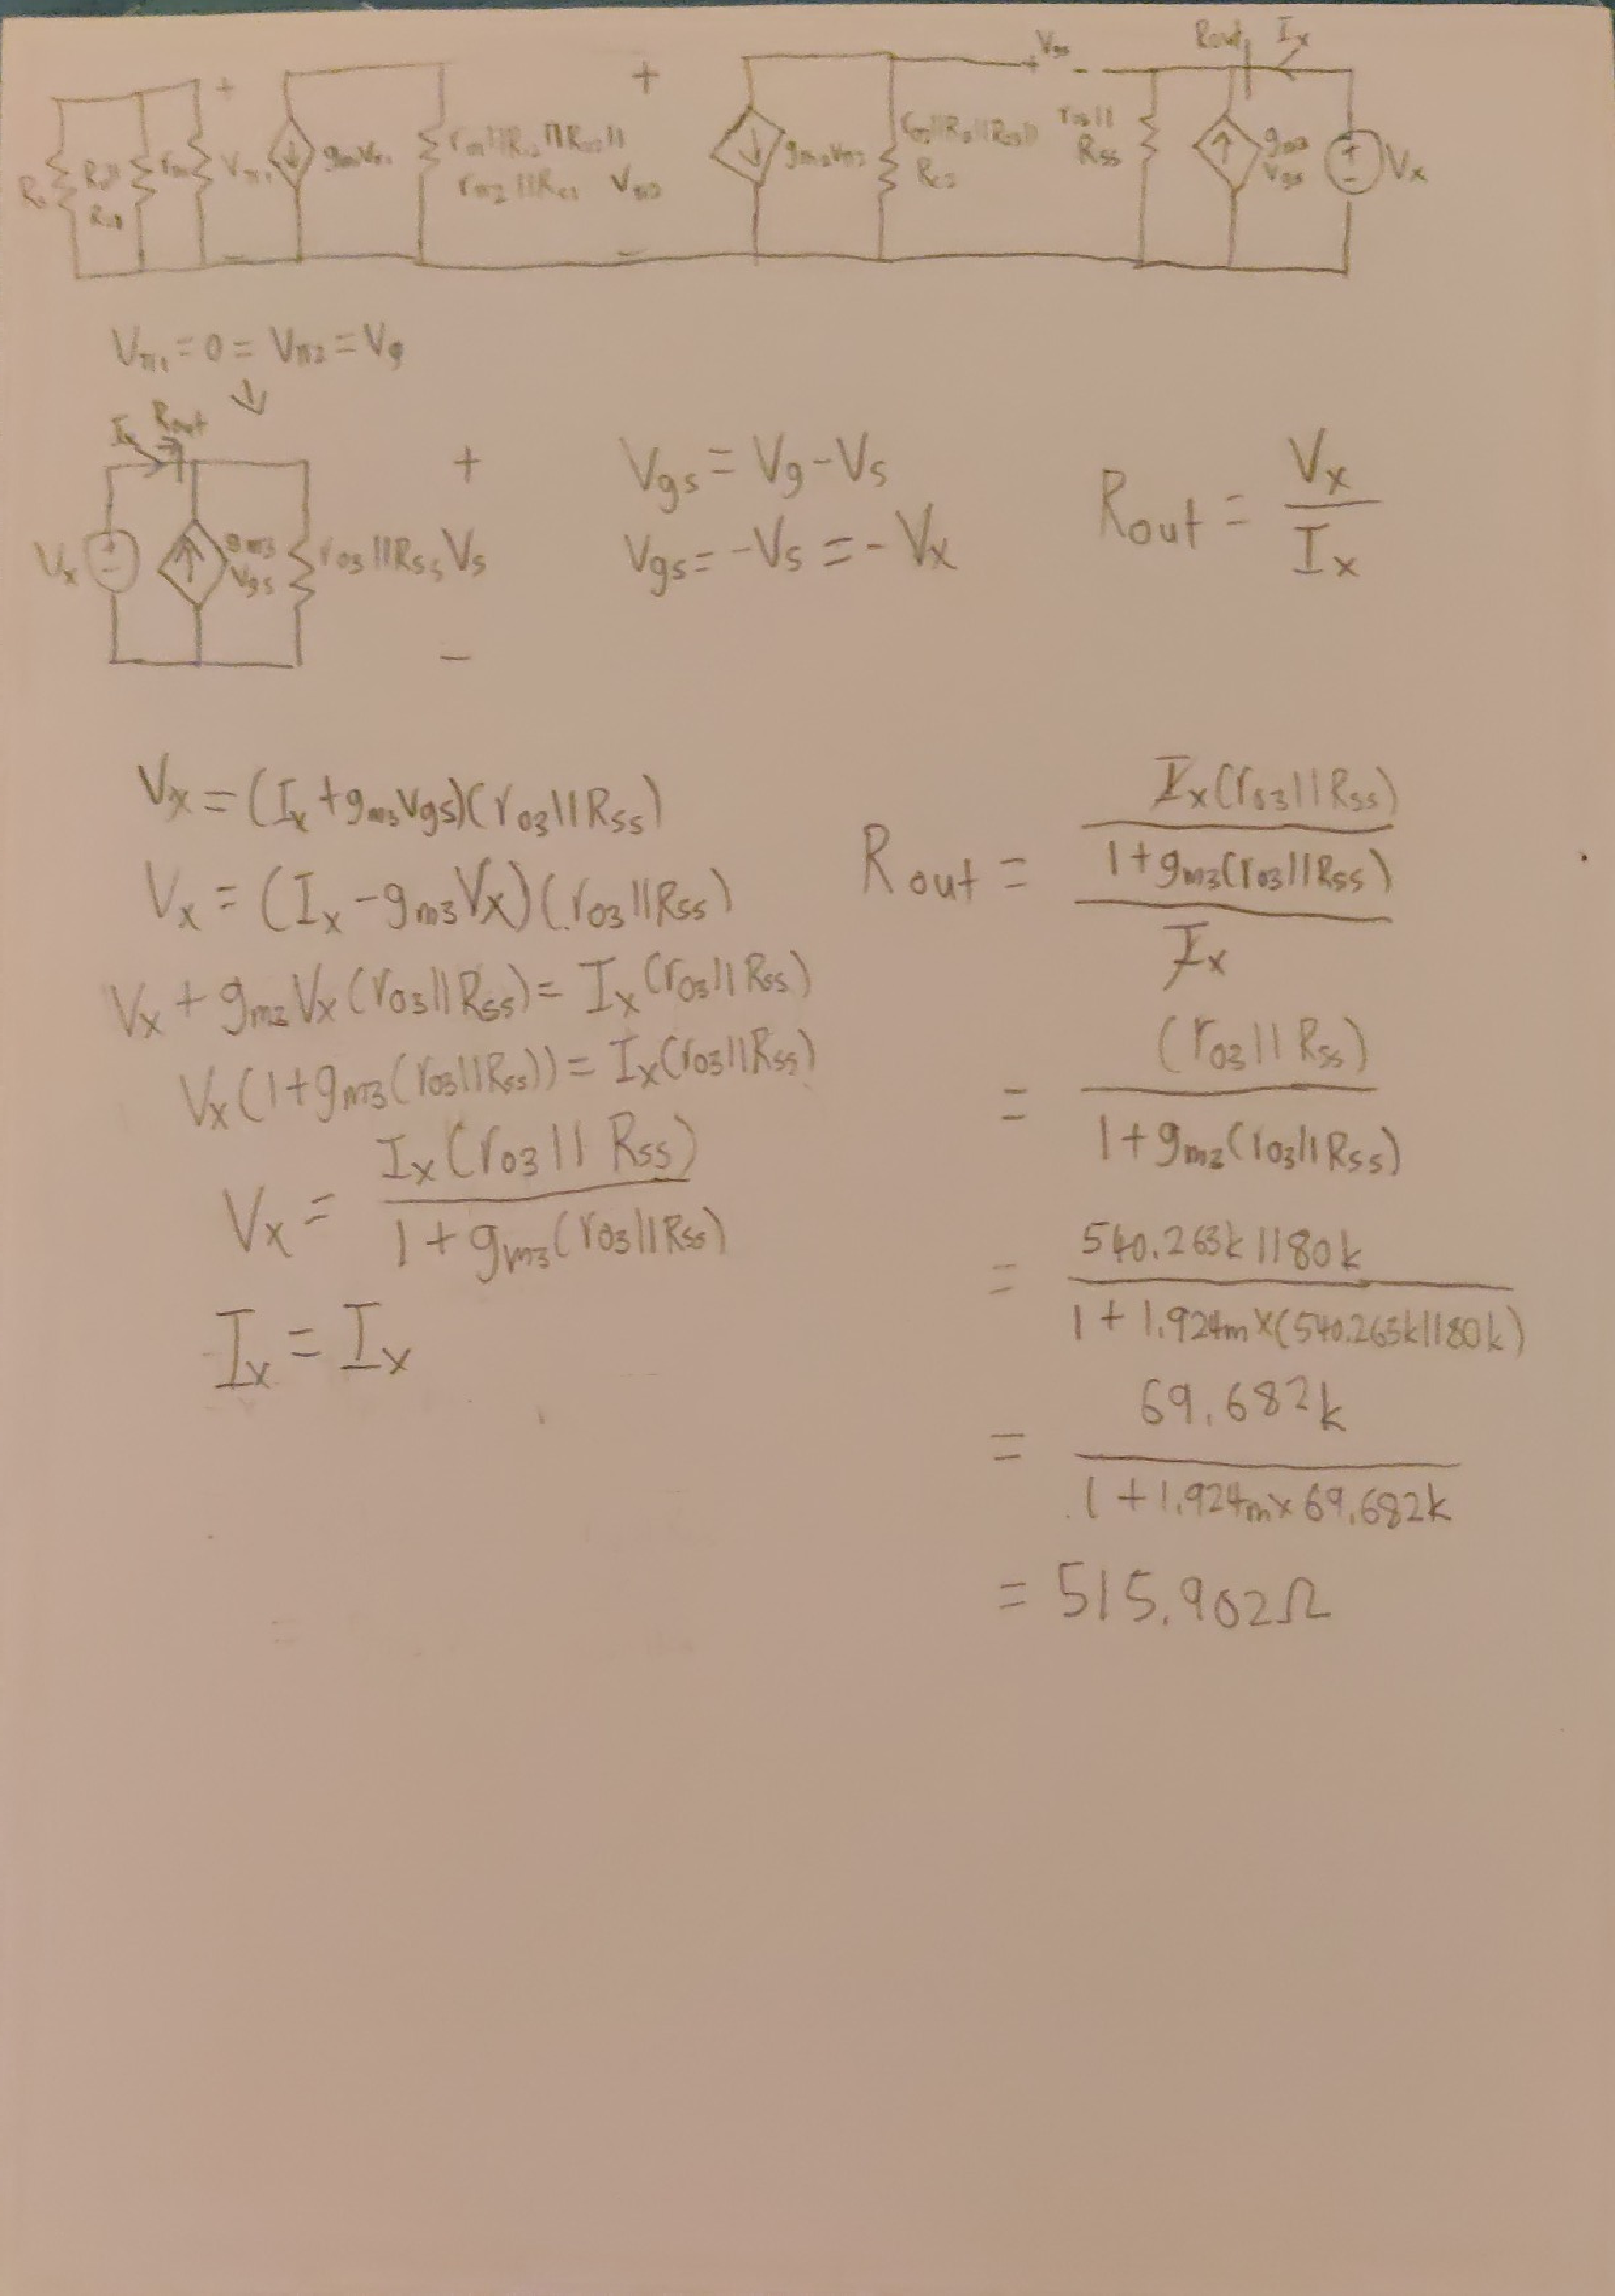
\includepdf[pages=1-]{img/output-resistance.pdf}

\section{Operating Regions}

Other than the gain of the amplifier, the transistors must also be operating in the correct region.
For a BJT to act as an amplifier, it must be operating in the forward active region.
When $V_{E} < V_{B} < V_{C}$, a BJT is in forward active region.
For a FET to act as an amplifier, it must be operating in the saturation region.
When $V_{DS} \ge V_{DS}(sat)$ and $V_{GS} > V_{TH}$ where $V_{DS}(sat) = V_{GS} - V_{TN}$, a FET is in saturation region.

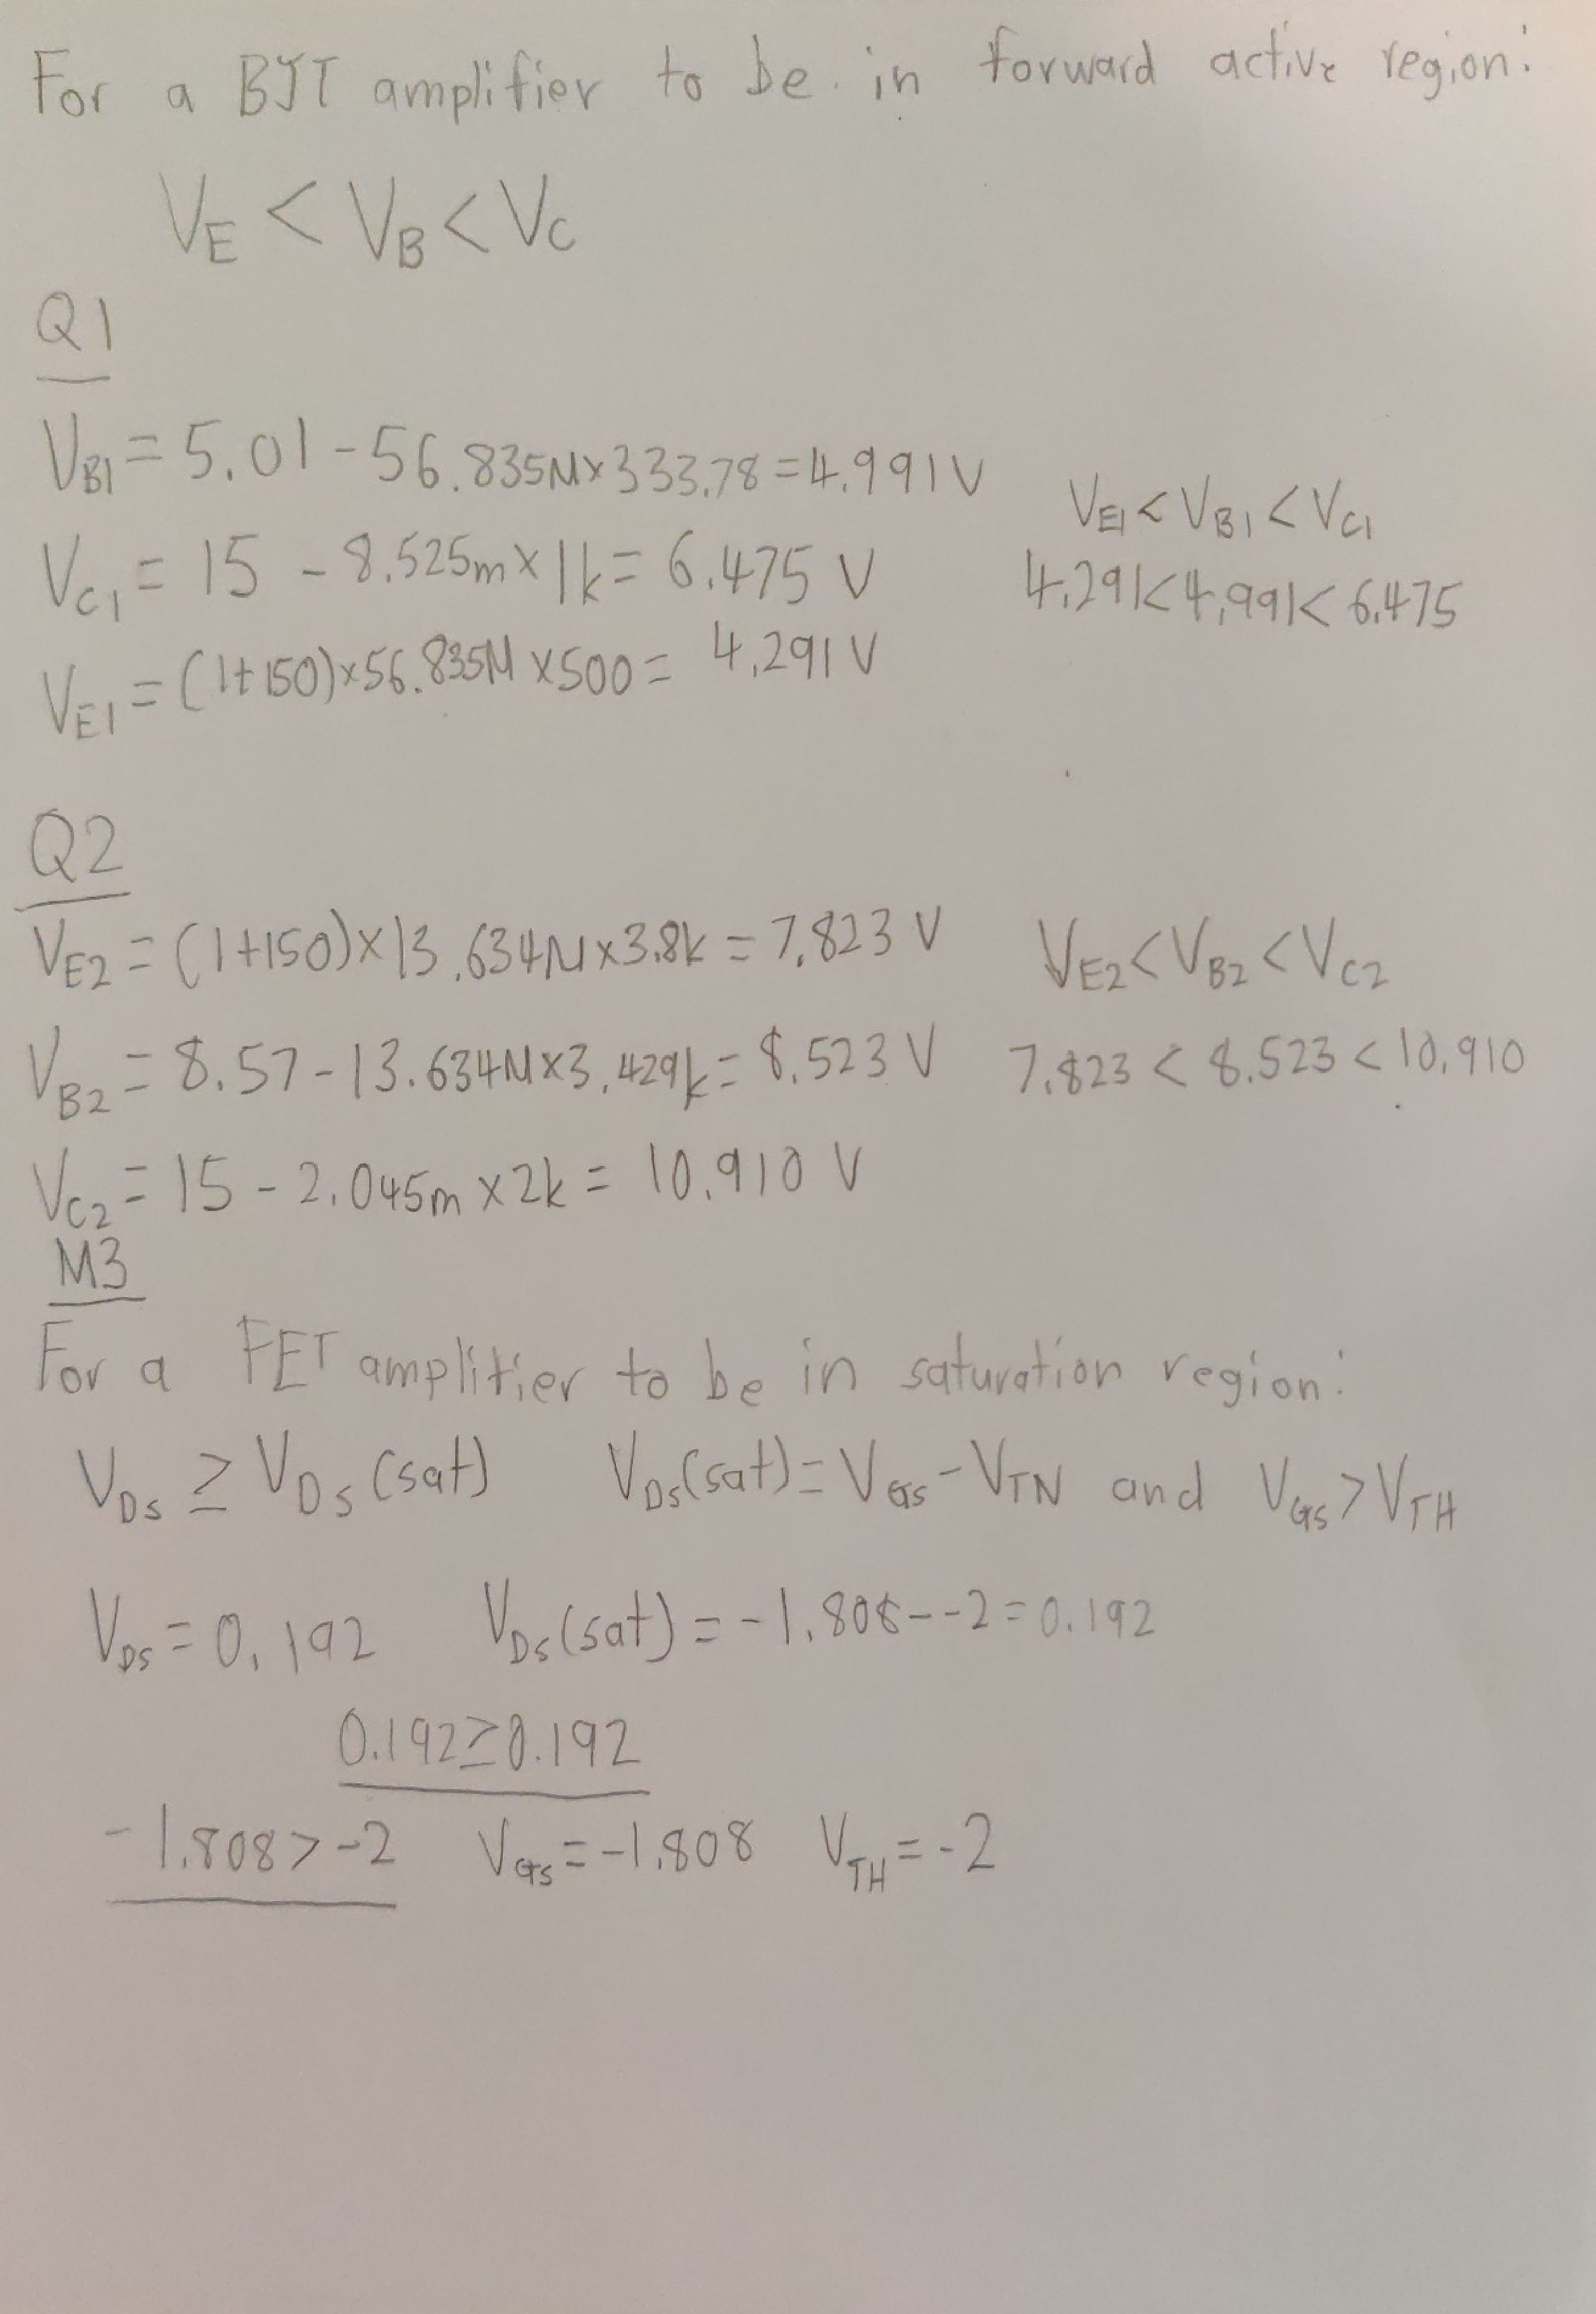
\includepdf{img/operating-region.pdf}

\section{Simulation and Calculated DC Analysis}
\label{sec:dc-analysis}

To double-check the calculations made, the amplifier design is created in LTSpice and simulated.
The transistor input voltage and current is recorded.
Table \ref{tab:sim-cal-dc-values} shows the difference between the simulated and calculated values.

\begin{table}[H]
    \caption{Table Showing Calculated and Simulated DC Values}
    \label{tab:sim-cal-dc-values}
    \centering
    \begin{tabular}{ l l l}
        \hline
        Value Name & Calculated       & Simulation       \\
        \hline
        $I_{B1}$   & $56.835 \mu{A}$  & $53.676 \mu{A}$  \\
        $I_{C1}$   & $8.525 mA$       & $8.267 mA$       \\
        $I_{E1}$   & $8.582 A$        & $8.321 mA$       \\
        $V_{B1}$   & $4.991 V$        & $4.989 V$        \\
        $V_{C1}$   & $6.475 V$        & $6.733 V$        \\
        $V_{E1}$   & $4.291 V$        & $4.161 V$        \\
        \hline
        $I_{B2}$   & $13.634 \mu{A}$  & $12.999 \mu{A}$  \\
        $I_{C2}$   & $2.045 mA$       & $2.023 mA$       \\
        $I_{E2}$   & $2.059 mA$       & $2.036 mA$       \\
        $V_{B2}$   & $8.523 V$        & $8.527 V$        \\
        $V_{C2}$   & $10.910 V$       & $10.955 V$       \\
        $V_{E2}$   & $7.823 V$        & $7.735 V$        \\
        \hline
        $I_{D}$    & $185.095 \mu{A}$ & $184.112 \mu{A}$ \\
        $V_{G}$    & $13 V$           & $13 V$           \\
        $V_{D}$    & $15 V$           & $15 V$           \\
        $V_{S}$    & $14.808 V$       & $14.729 V$       \\
        \hline
    \end{tabular}
\end{table}

A small discrepancies are noted between the calculated values and simulated values for BJT.
This is due to the differences in simulation parameters for the BJT.
The $V_{BE}$ of the simulation is different from the ones used for calculation.
This is due to the built-in $I_{s}$ current parameter of the BJT.
The fixed saturation current forces the $V_{BE}$ value to be different.

Both calculated and simulated values for FET are similar.
However, there are still minor differences.
The differences aren't big as they are only a few decimal places apart.
This is probably due to the rounding of the values during calculation.

\begin{figure}[H]
    \centering
    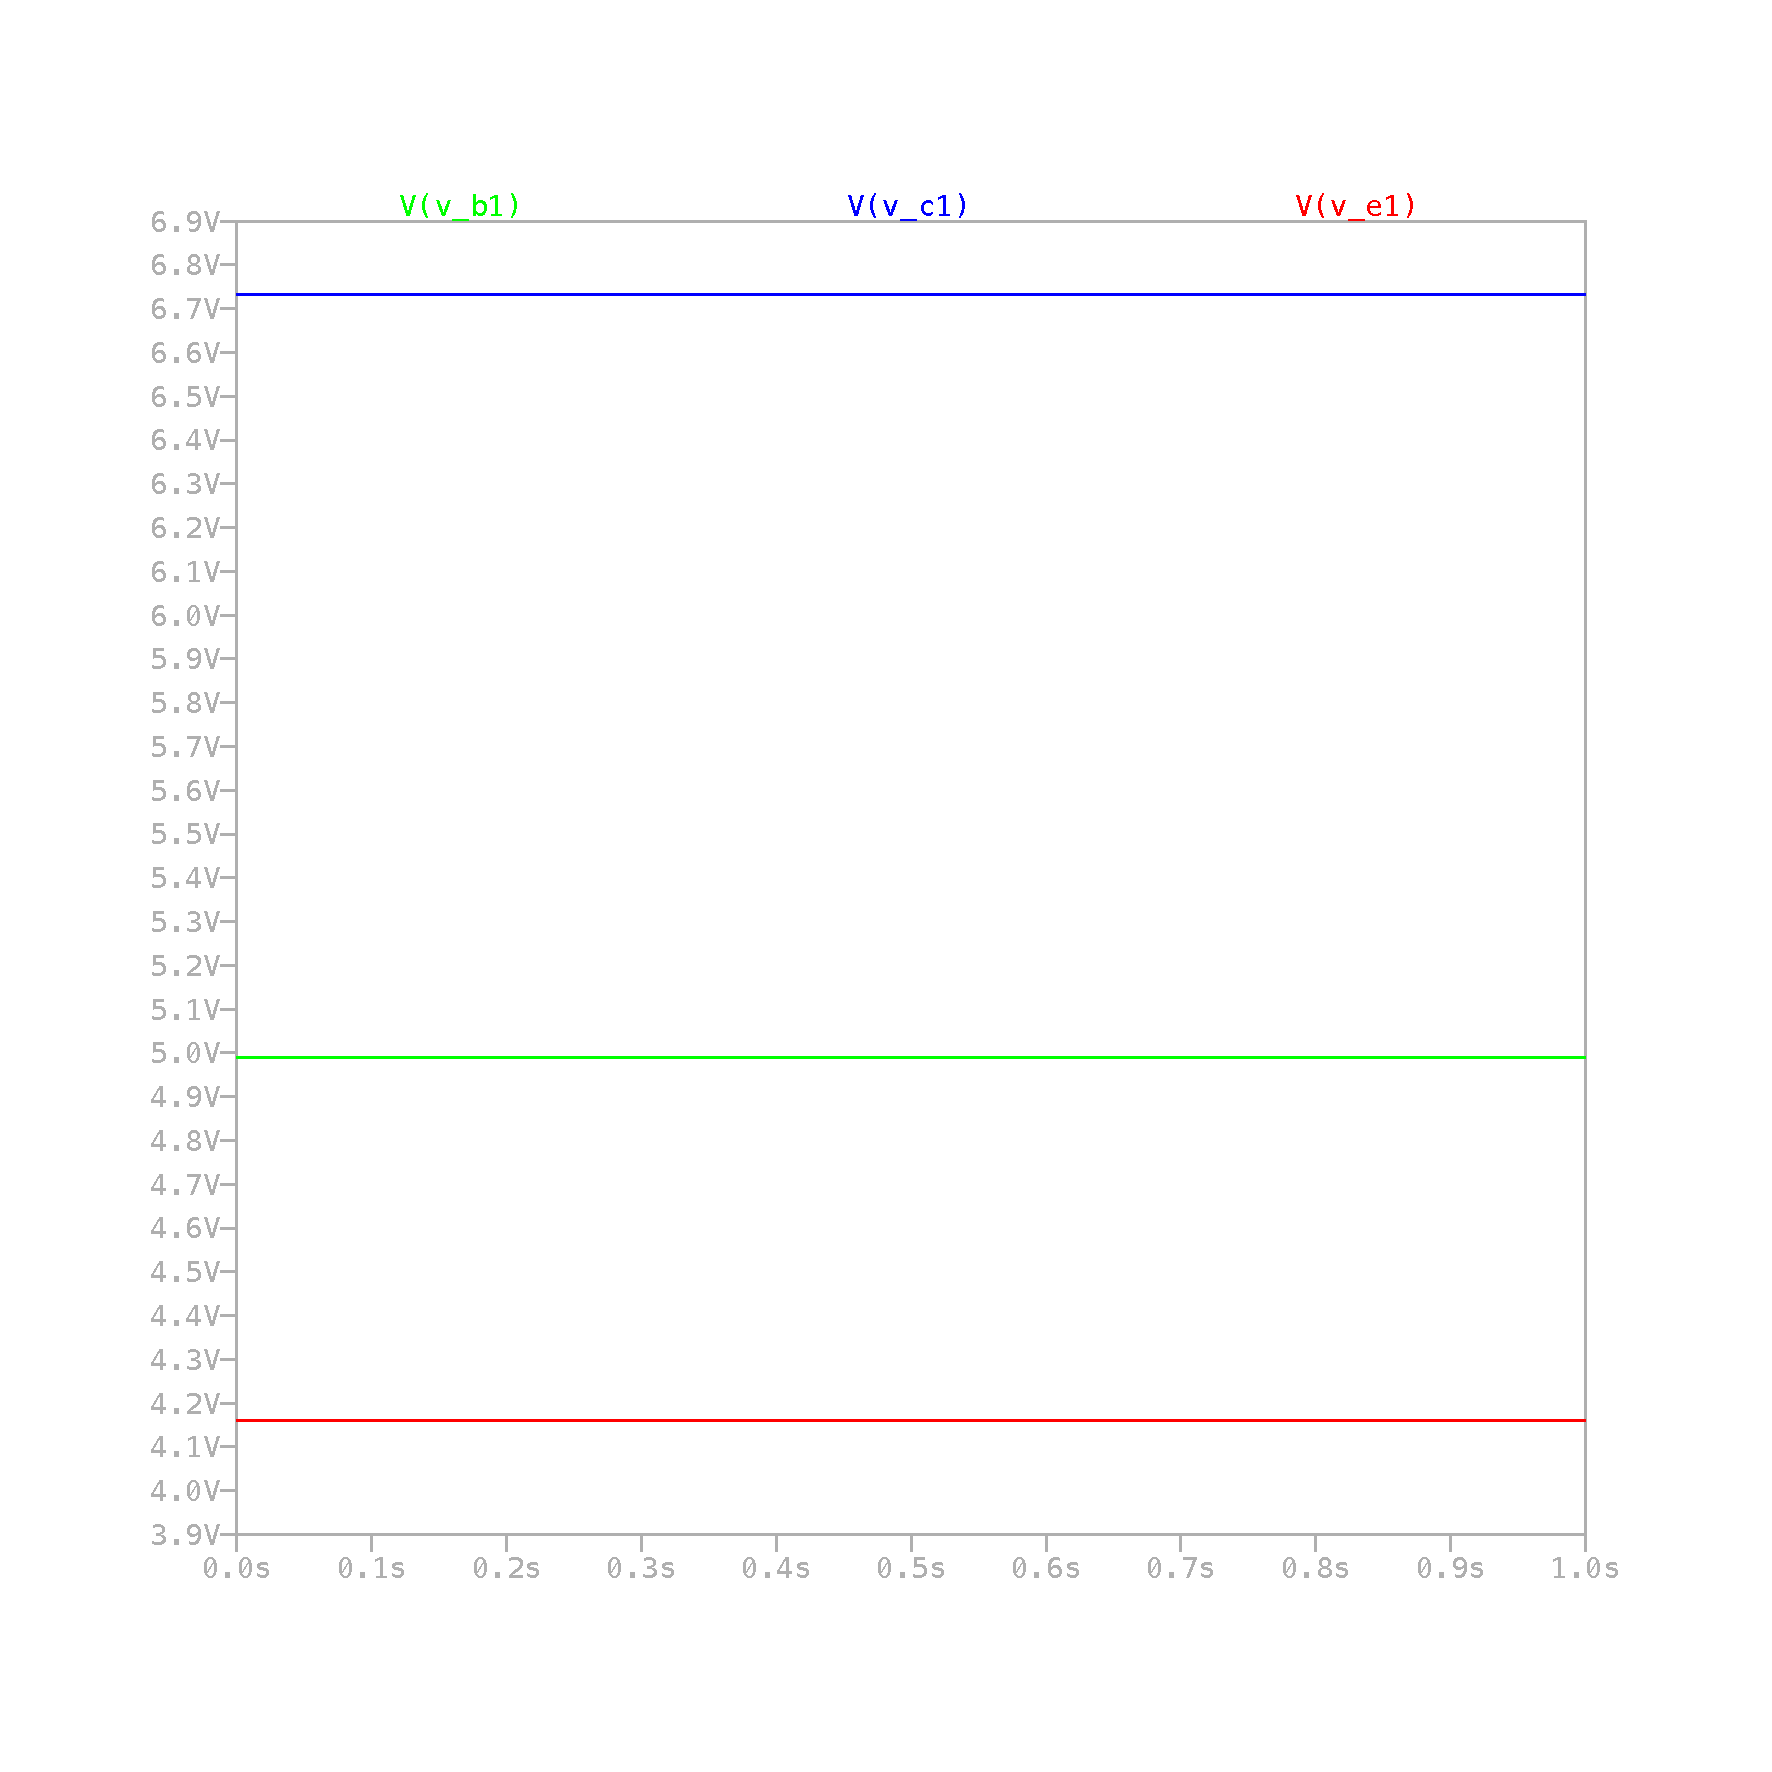
\includegraphics[height=0.4\textheight,trim={30mm 30mm 30mm 30mm}]{img/Amplifier Design Q1 V.pdf}
    \caption{DC Voltages for Q1}
    \label{fig:dc-v-q1}
\end{figure}

\begin{figure}[H]
    \centering
    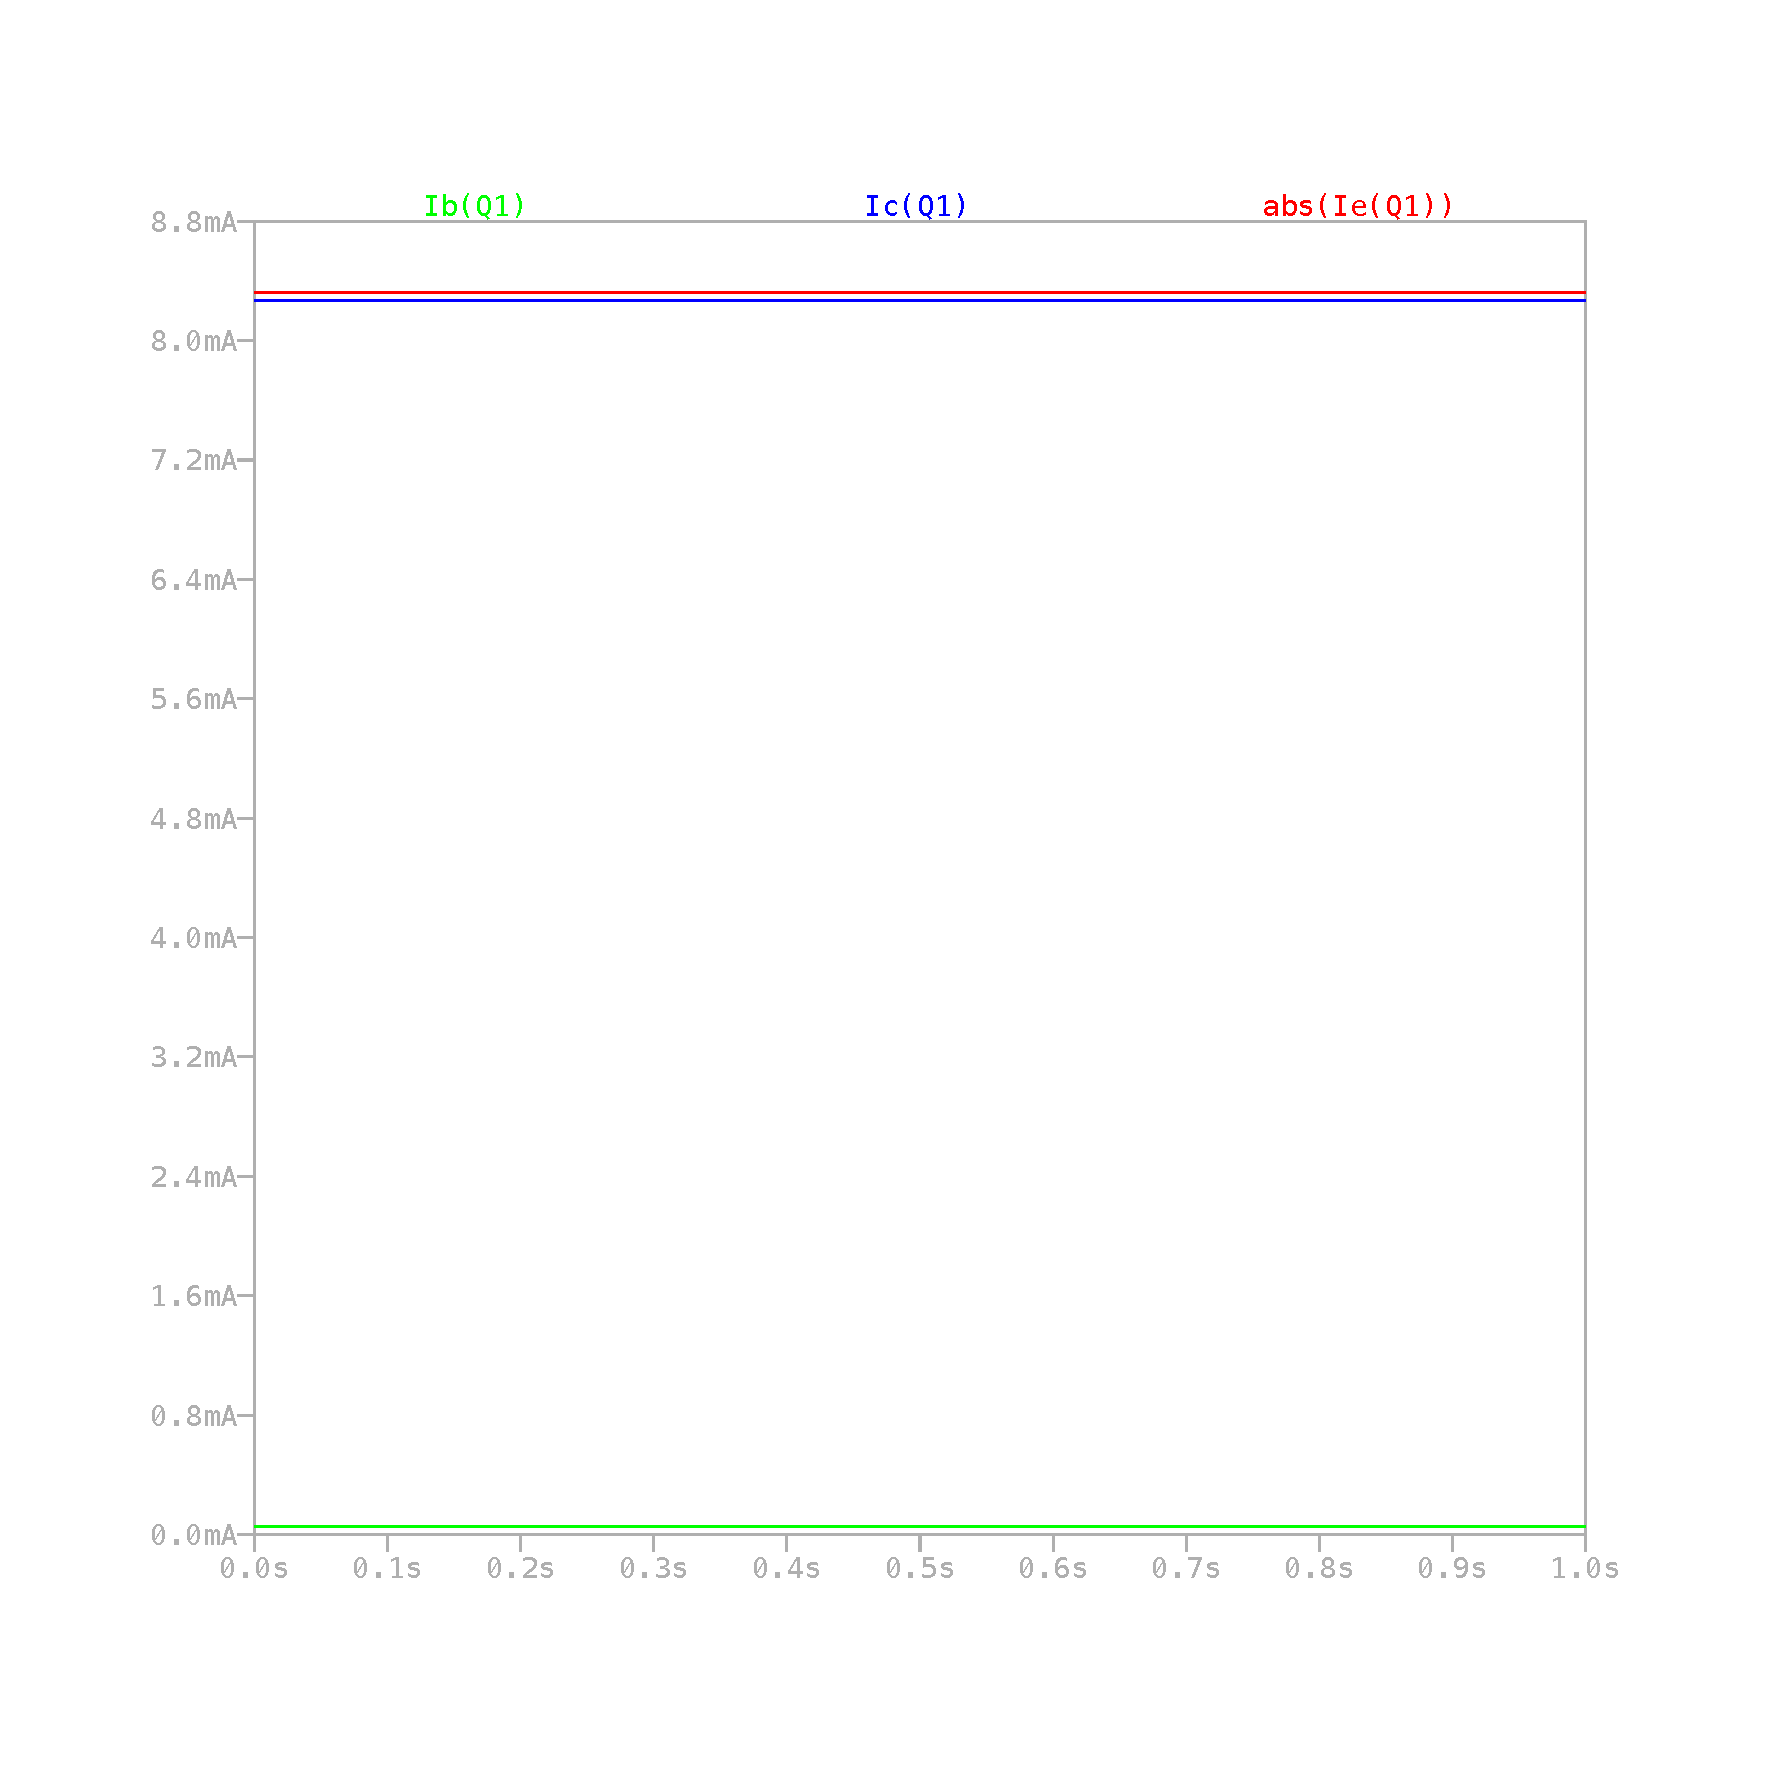
\includegraphics[height=0.4\textheight,trim={30mm 30mm 30mm 30mm}]{img/Amplifier Design Q1 I.pdf}
    \caption{DC Current for Q1}
    \label{fig:dc-i-q1}
\end{figure}

\begin{figure}[H]
    \centering
    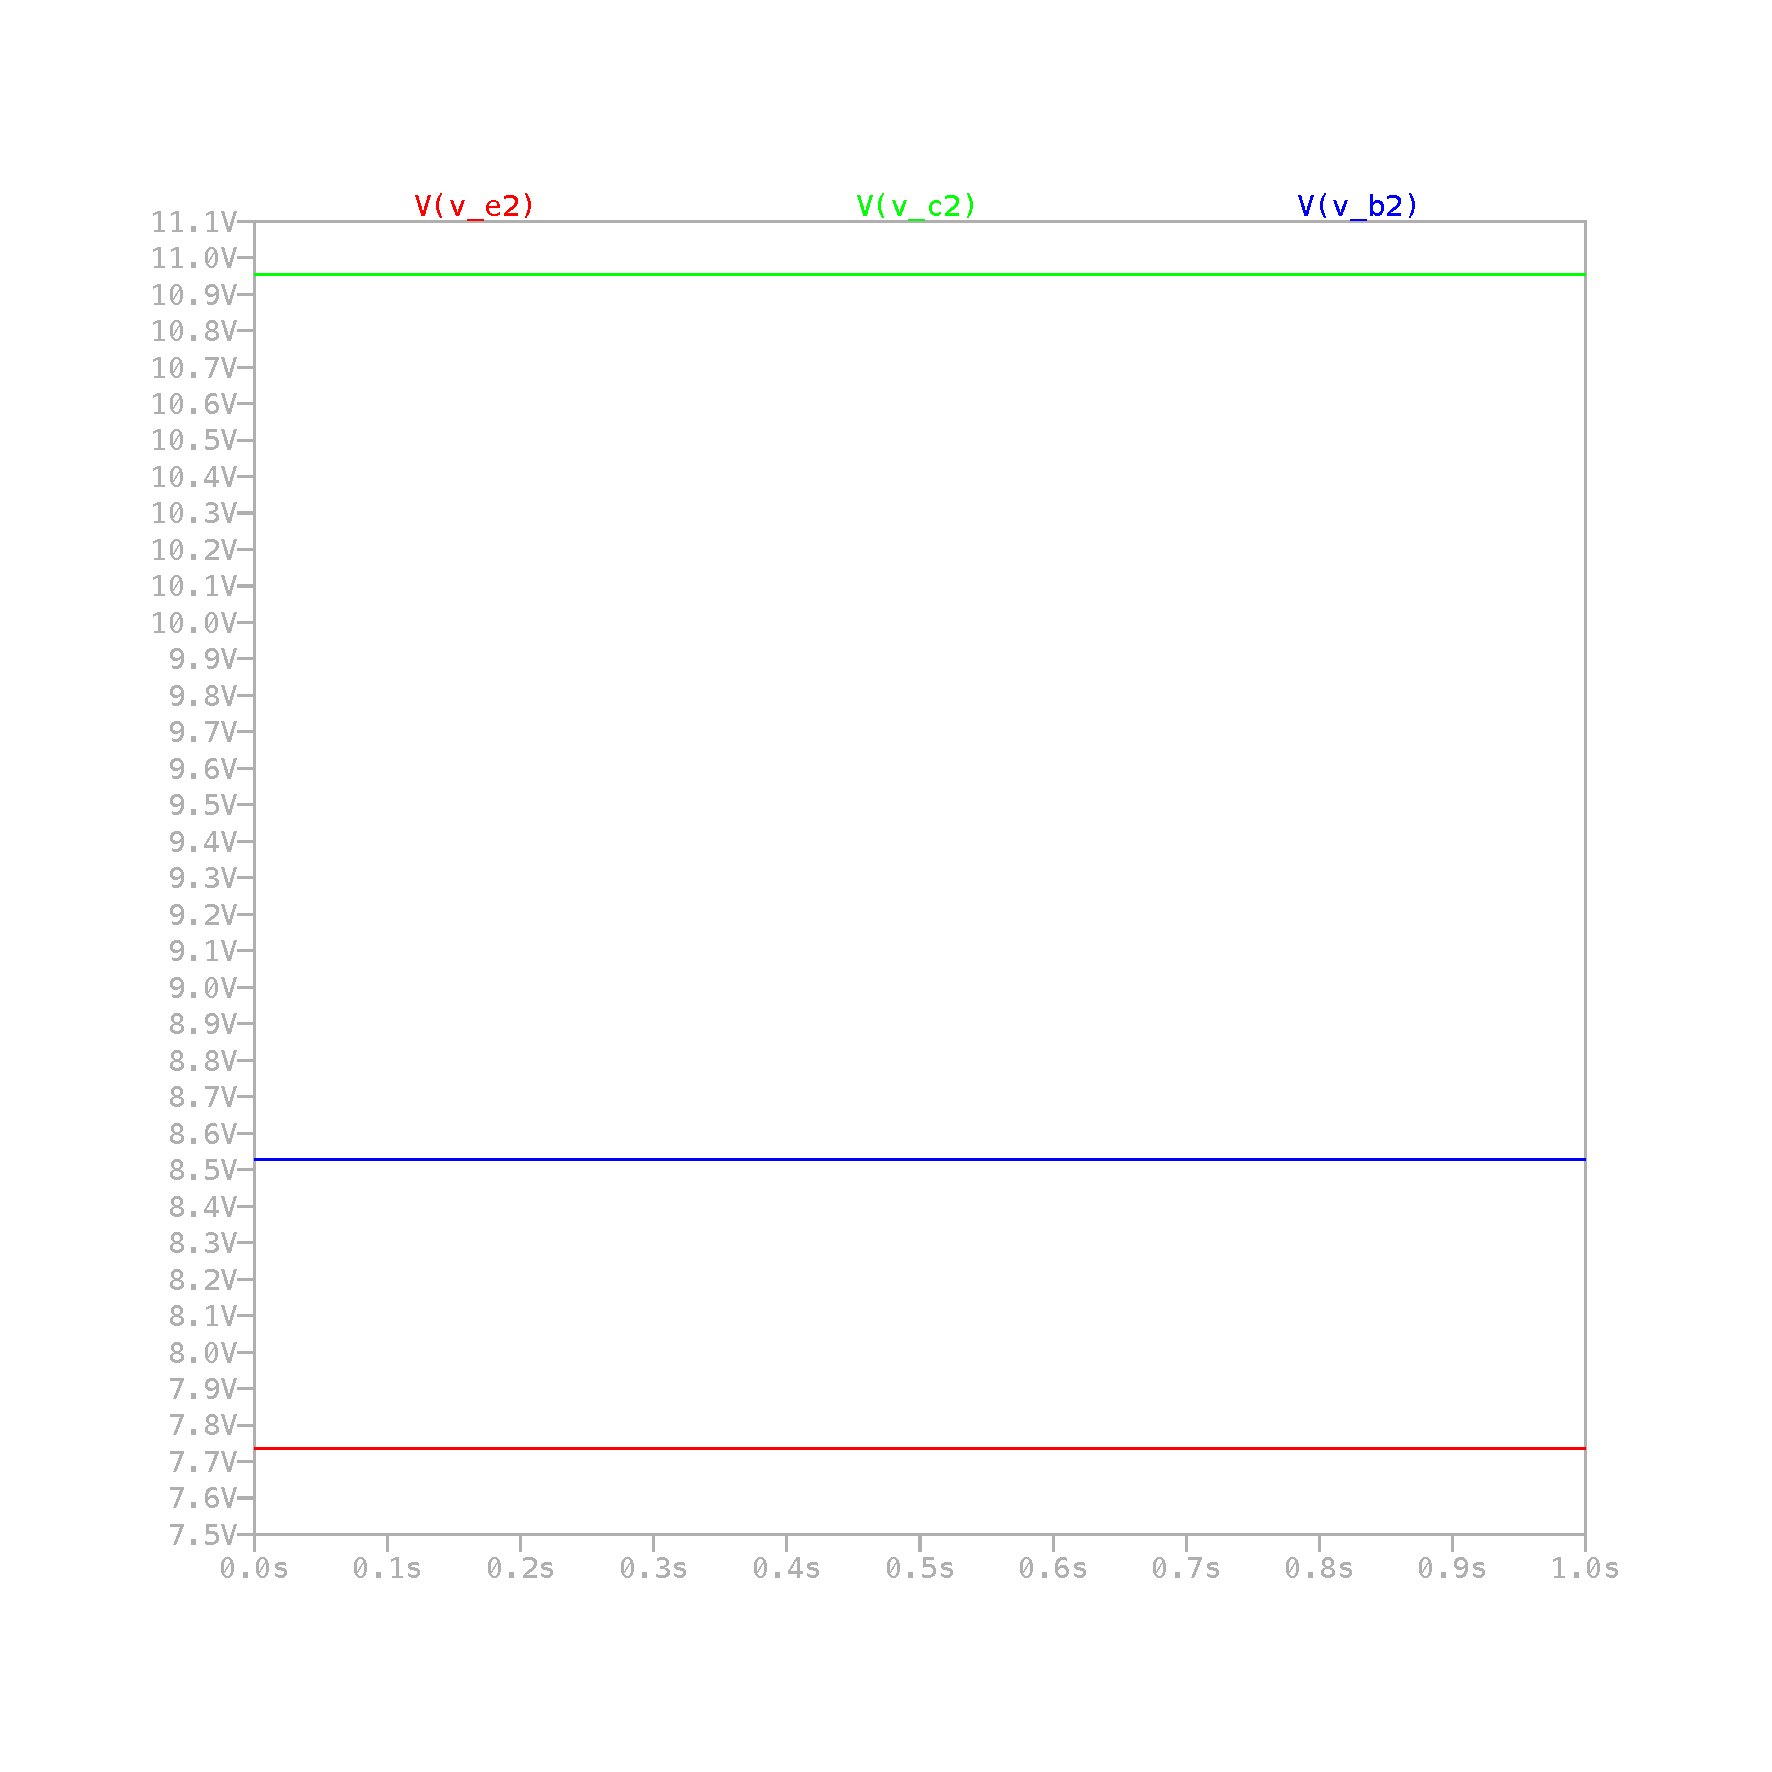
\includegraphics[height=0.4\textheight,trim={30mm 30mm 30mm 30mm}]{img/Amplifier Design Q2 V.pdf}
    \caption{DC Voltages for Q2}
    \label{fig:dc-v-q2}
\end{figure}

\begin{figure}[H]
    \centering
    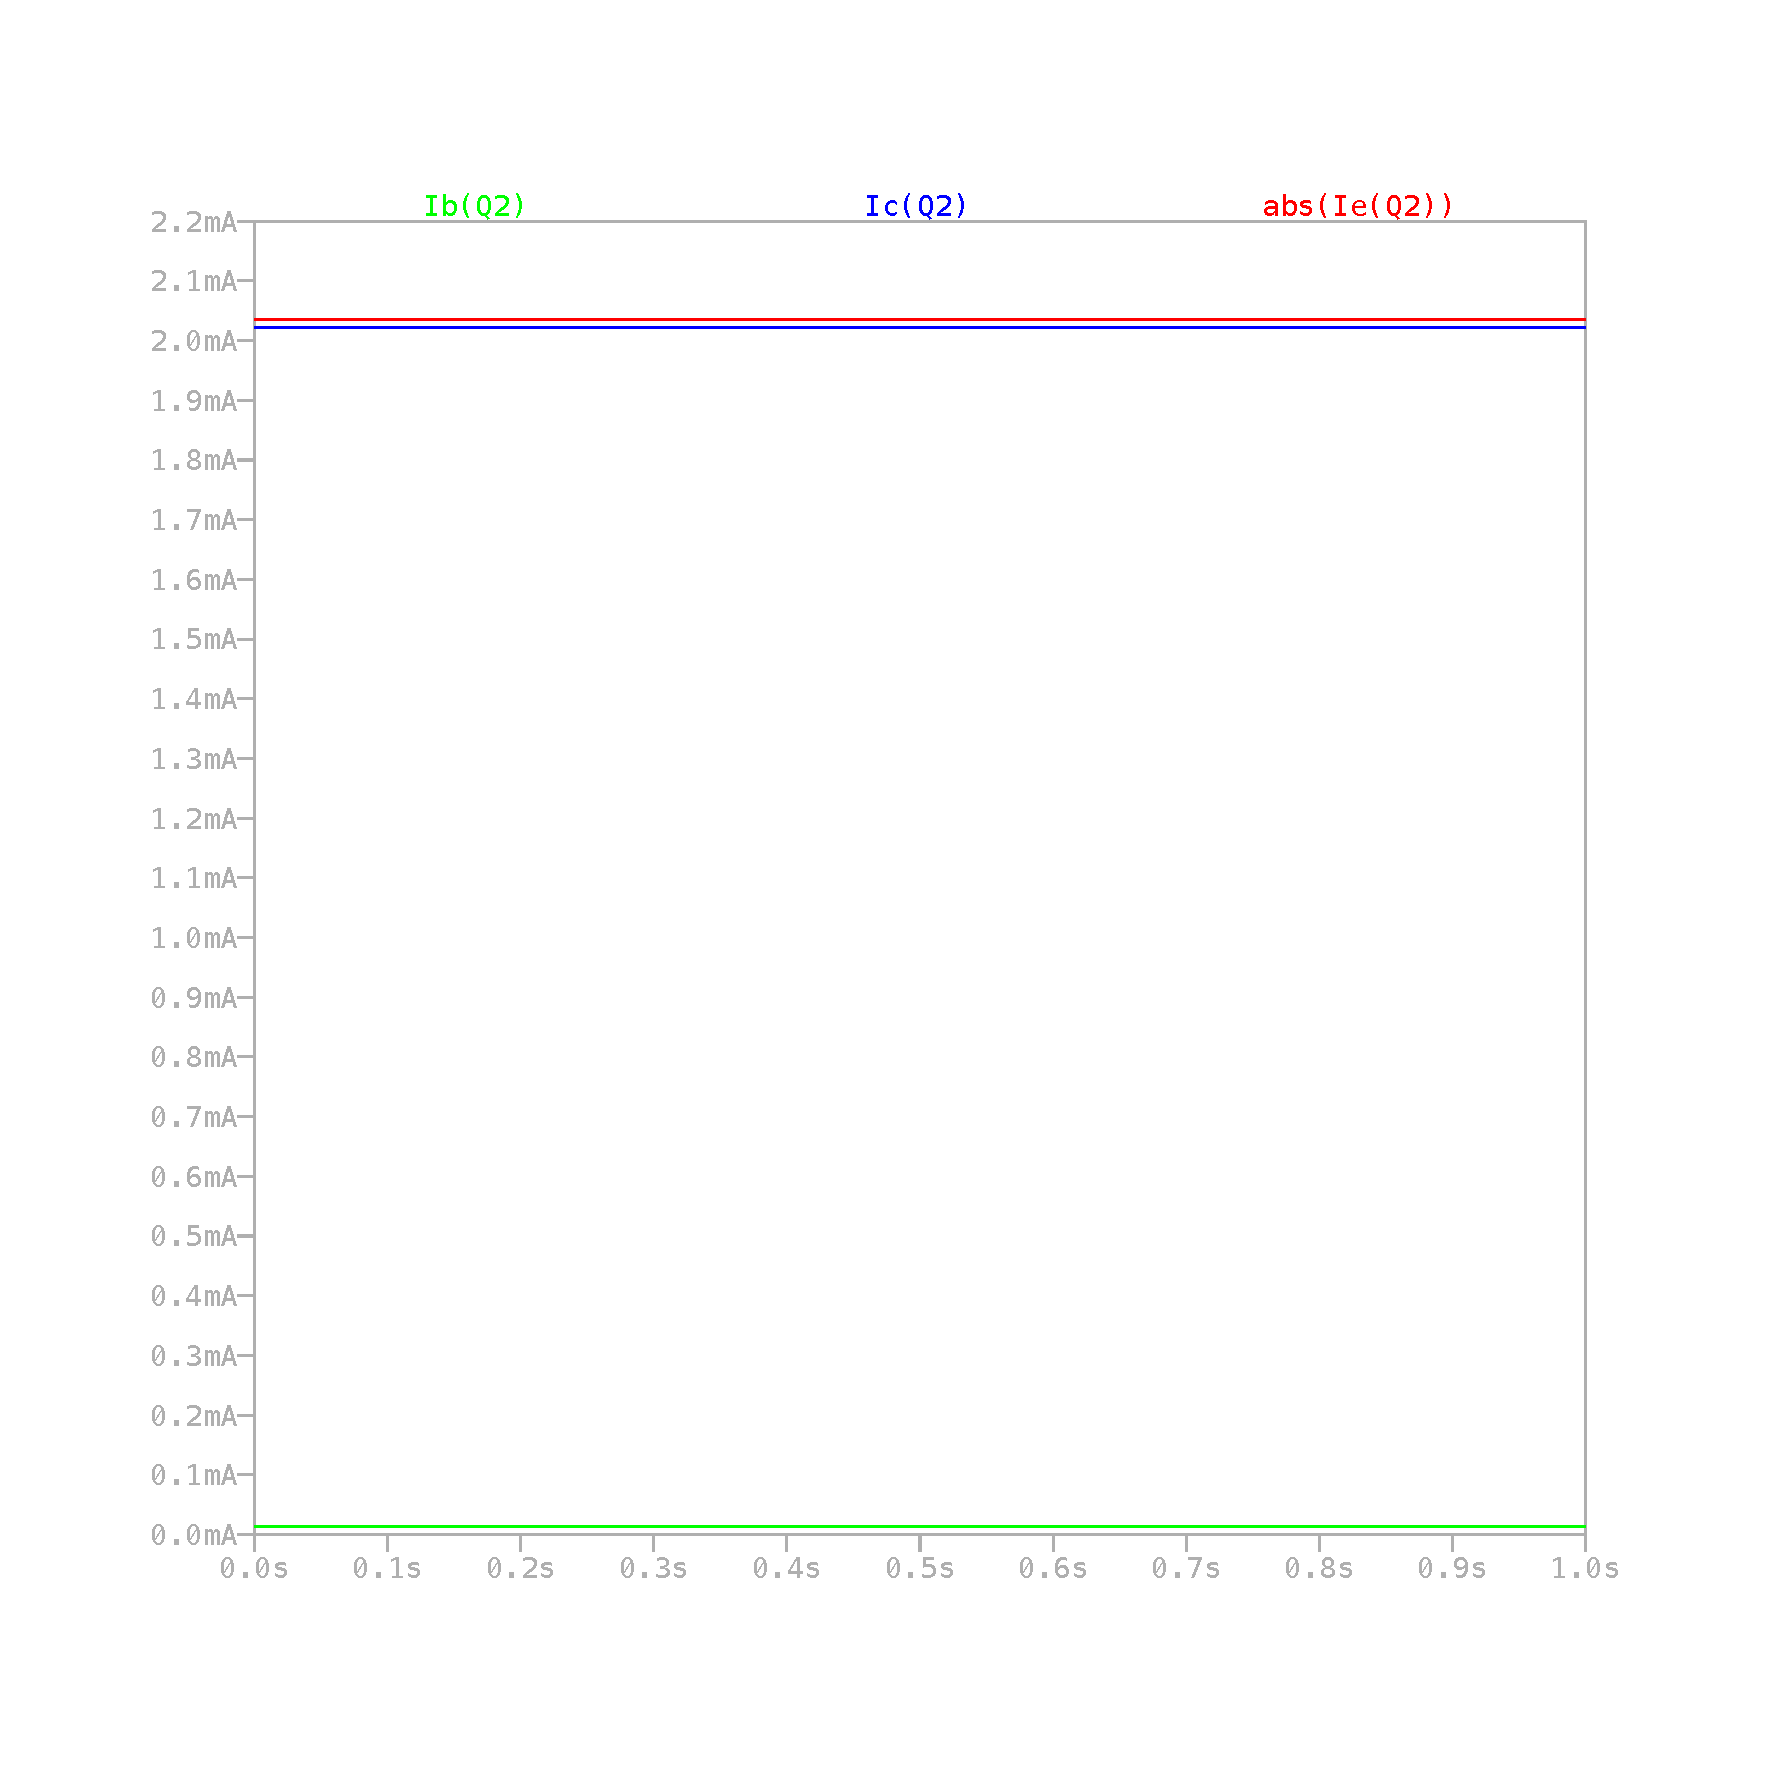
\includegraphics[height=0.4\textheight,trim={30mm 30mm 30mm 30mm}]{img/Amplifier Design Q2 I.pdf}
    \caption{DC Current for Q2}
    \label{fig:dc-i-q2}
\end{figure}

\begin{figure}[H]
    \centering
    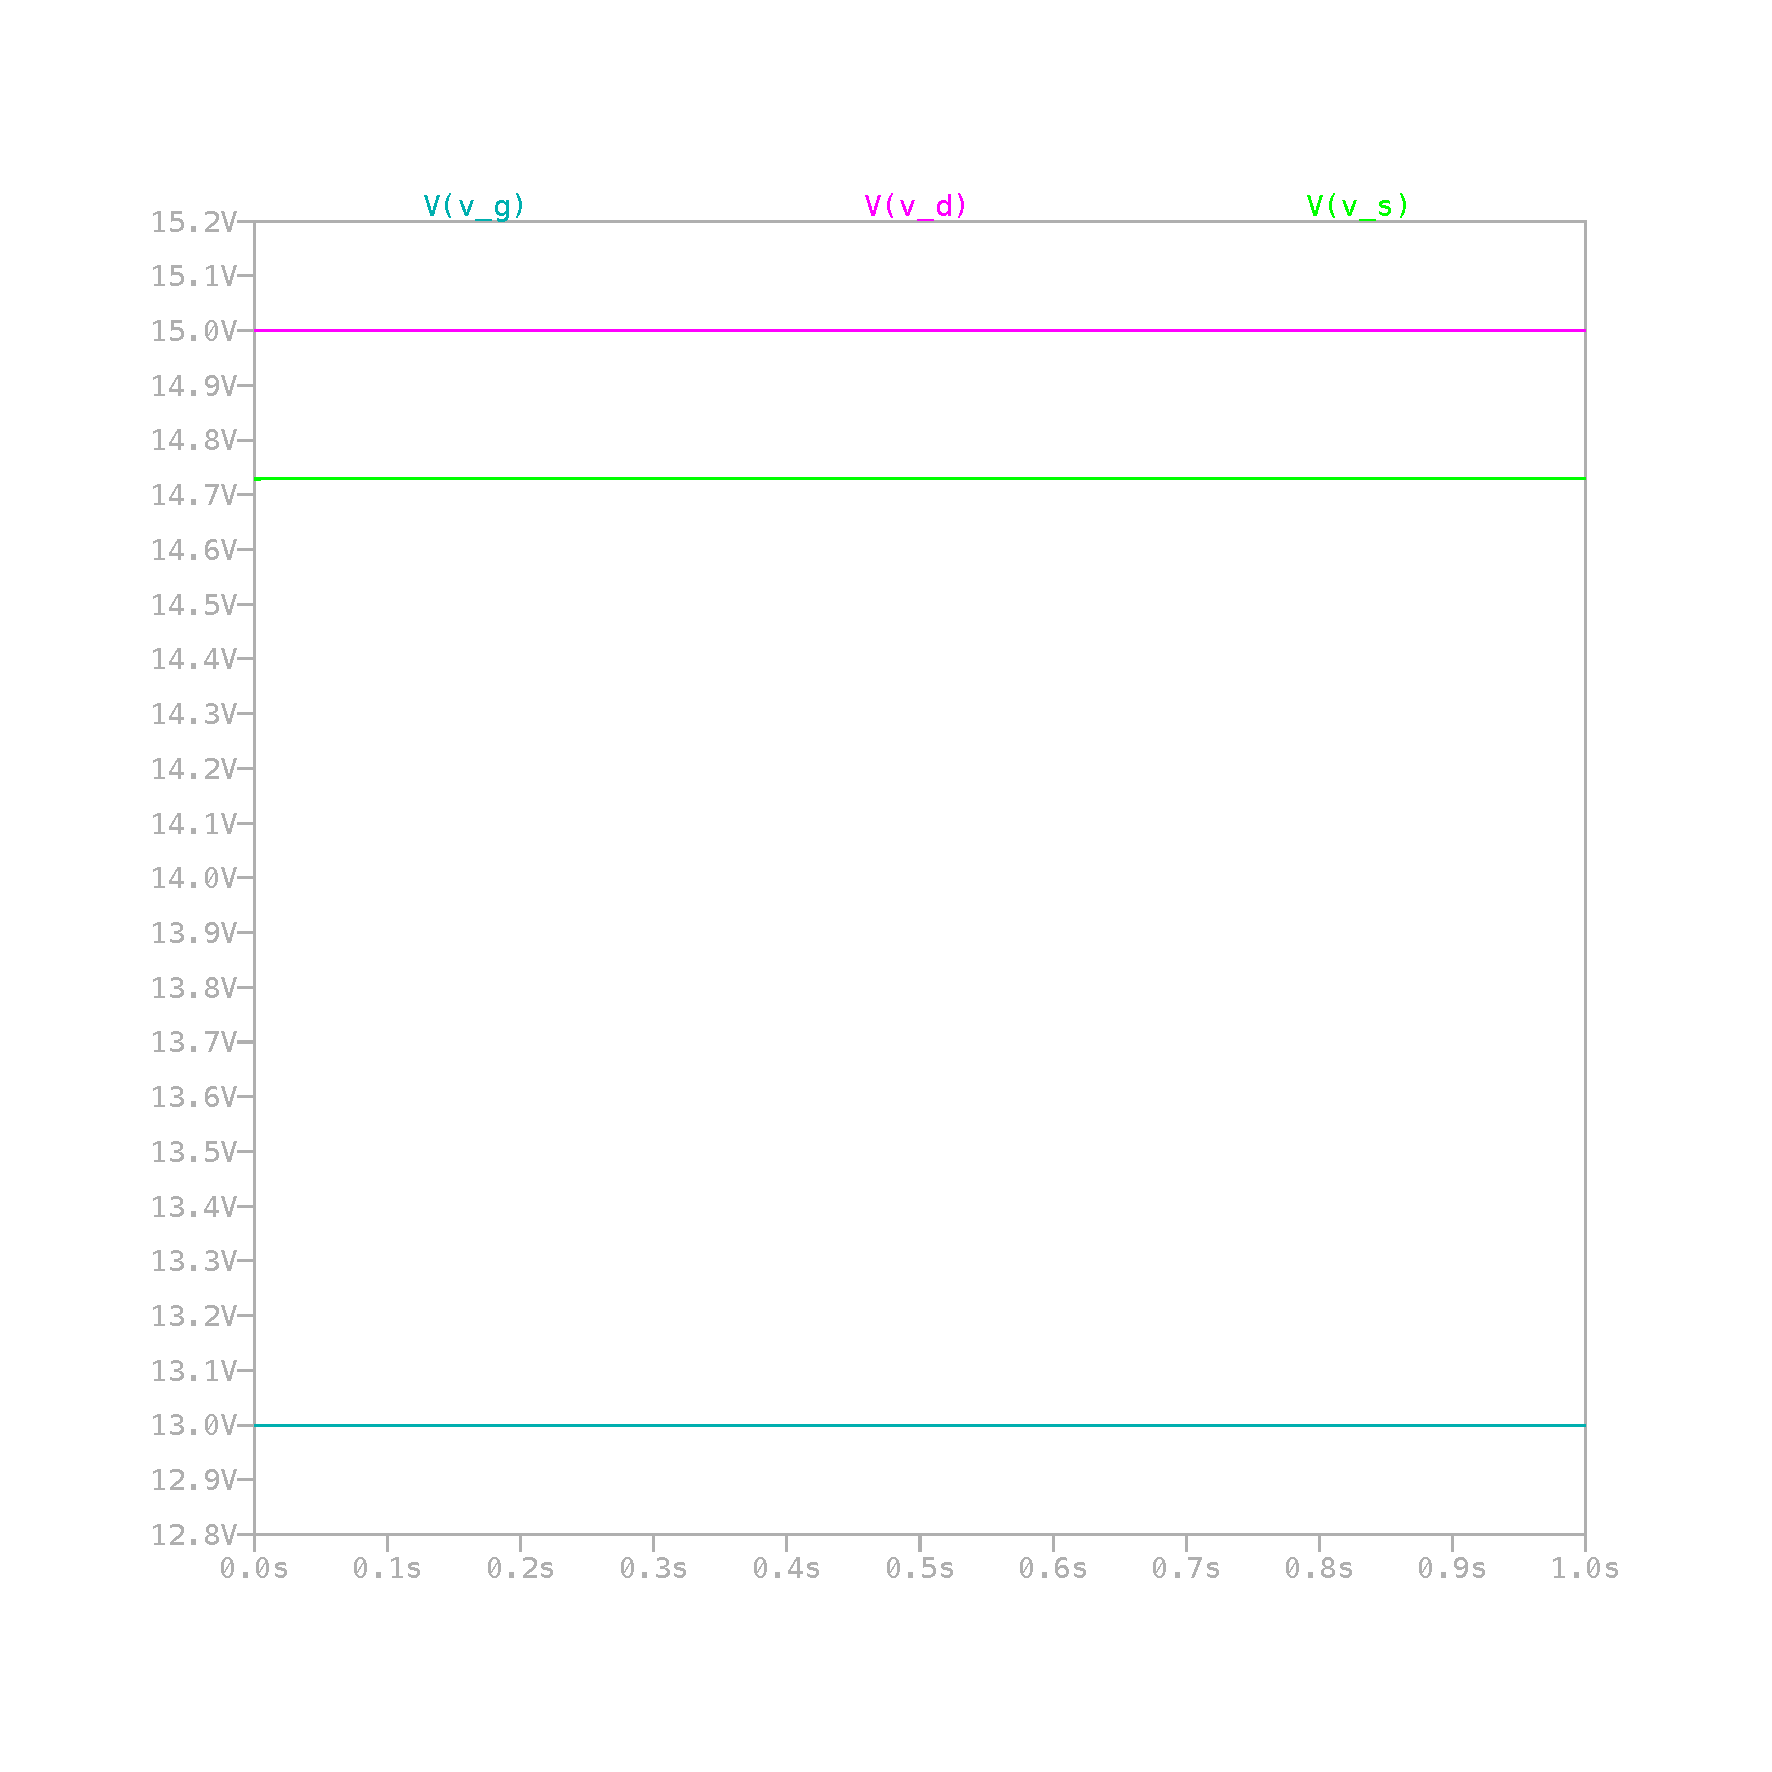
\includegraphics[height=0.4\textheight,trim={30mm 30mm 30mm 30mm}]{img/Amplifier Design M3 V.pdf}
    \caption{DC Voltages for M3}
    \label{fig:dc-v-m3}
\end{figure}

\begin{figure}[H]
    \centering
    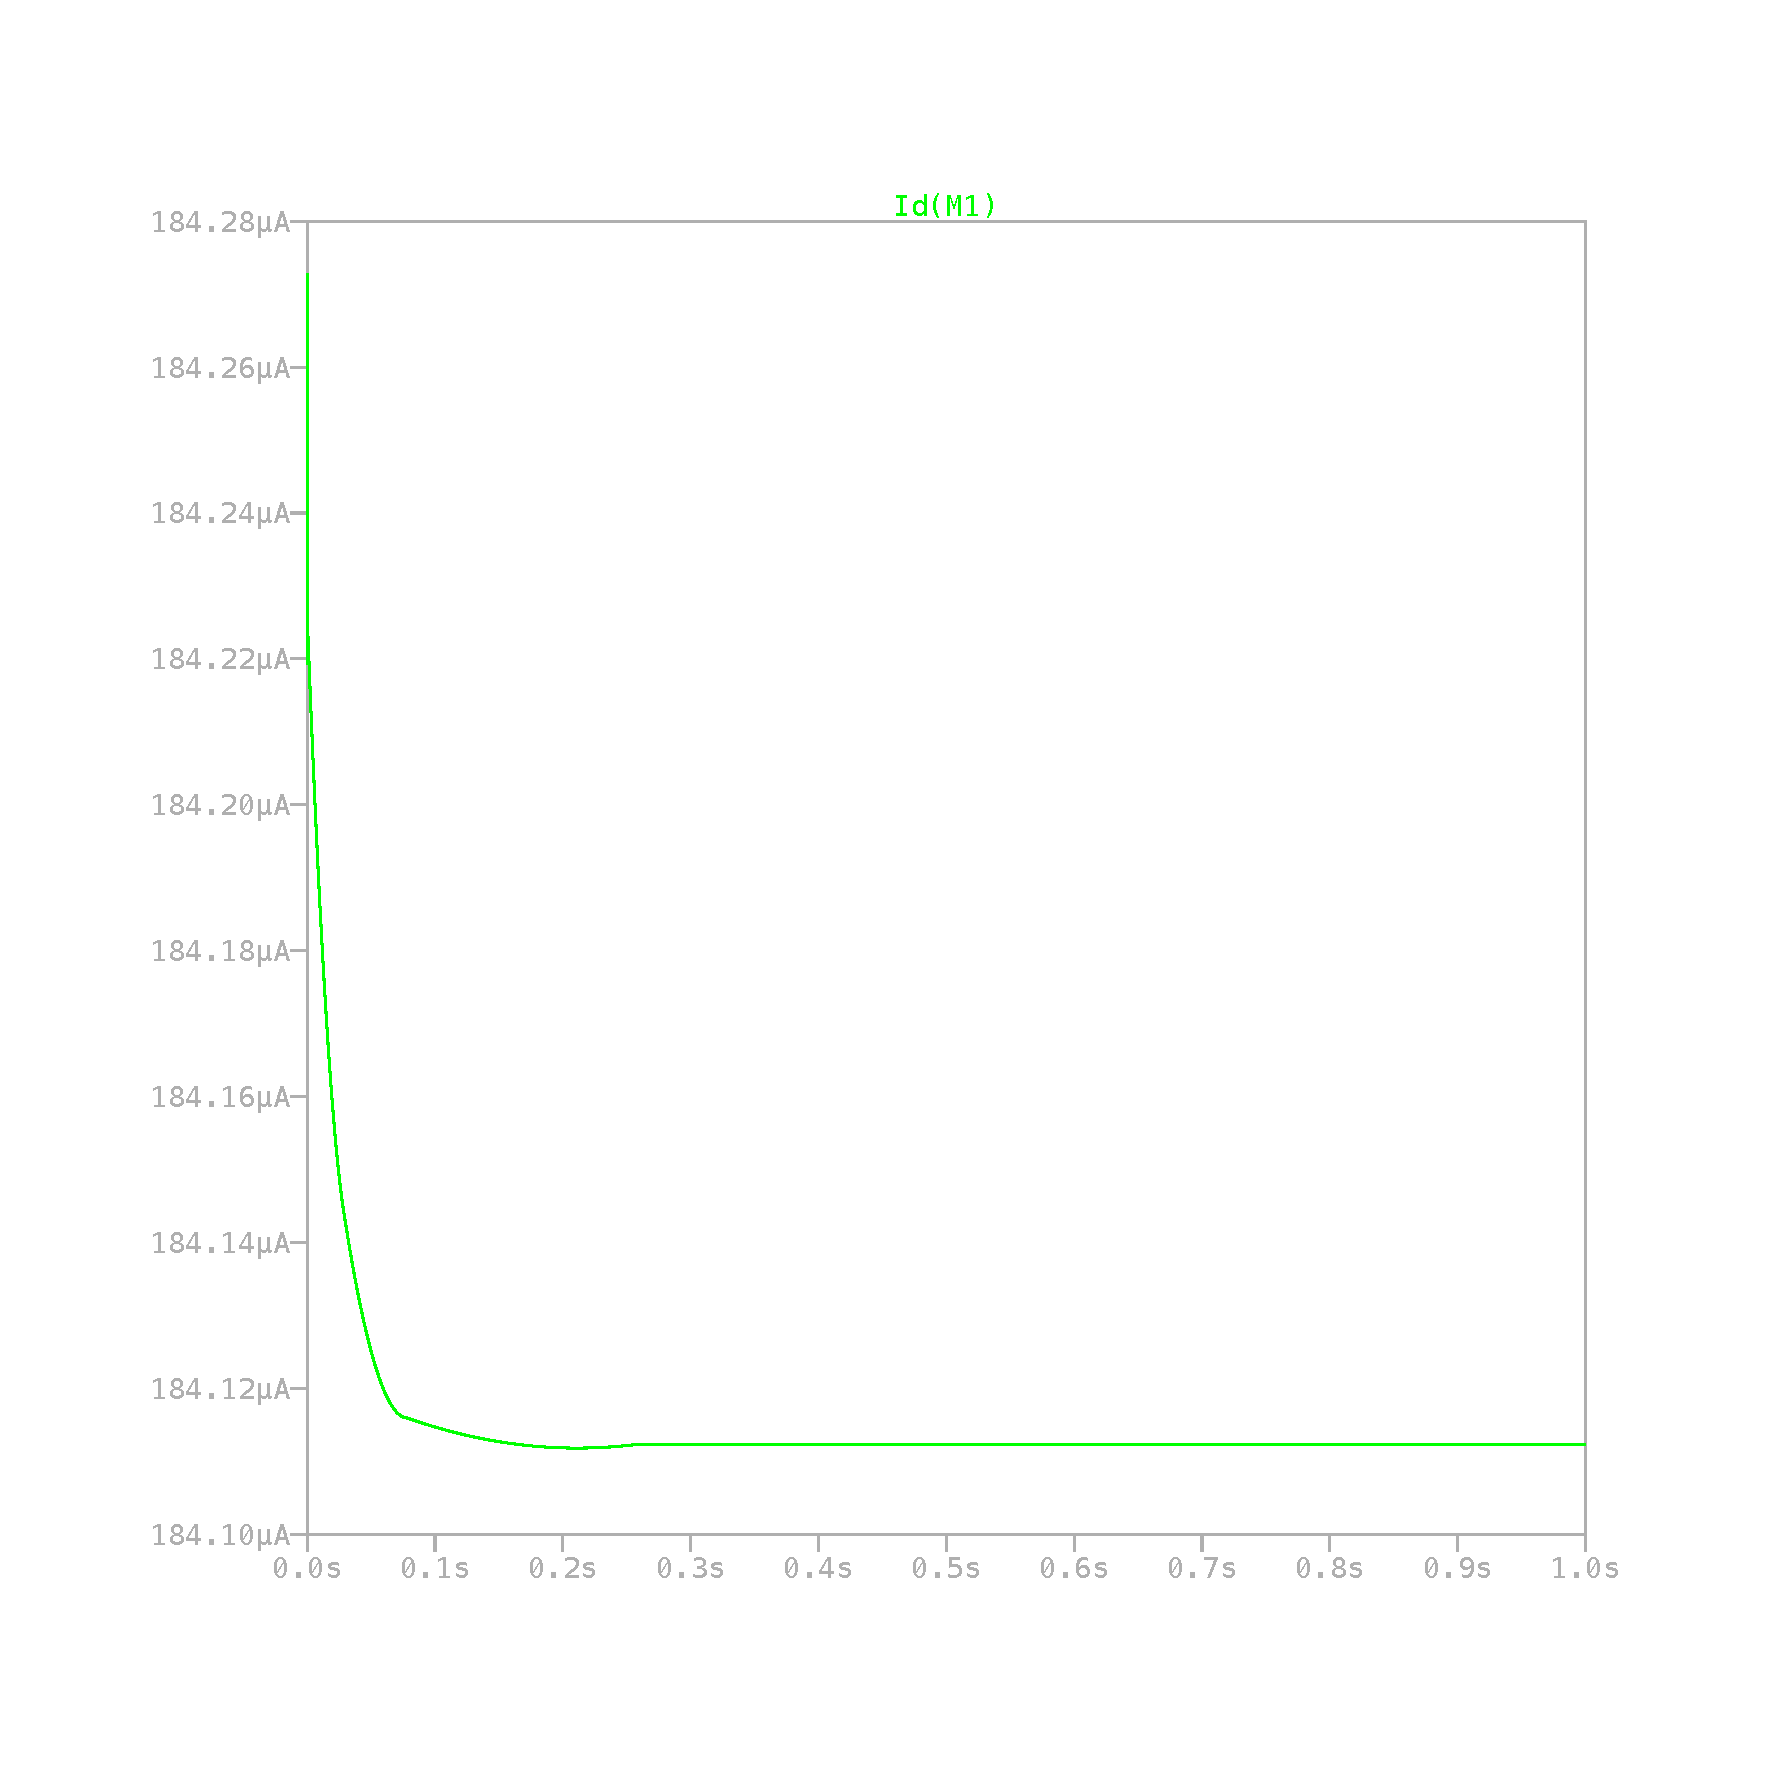
\includegraphics[height=0.4\textheight,trim={30mm 30mm 30mm 30mm}]{img/Amplifier Design M3 I.pdf}
    \caption{DC Current for M3}
    \label{fig:dc-i-m3}
\end{figure}

\section{AC Simulation}

The amplifier circuit is also simulated in AC.
This shows the amplifier response at different frequency.
The gain ($A_{v} = V_{o} / V_{in}$), input resistance $R_{in}$ and output resistance $R_{out}$ are measured.
Table \ref{tab:sim-cal-ac-values} shows the difference between calculated and simulated values.

\begin{table}[H]
    \caption{Table Showing Calculated and Simulated AC Values}
    \label{tab:sim-cal-ac-values}
    \centering
    \begin{tabular}{ l l l}
        \hline
        Value Name & Calculated       & Simulation       \\
        \hline
        $A_{v}$    & $67.537$         & $53.722$         \\
        $R_{in}$   & $192.977 \Omega$ & $197.190 \Omega$ \\
        $R_{out}$  & $515.902 \Omega$ & $727.989 \Omega$ \\
        \hline
    \end{tabular}
\end{table}

The circuit in the simulation meet the design requirements.
However, the values obtained are different from the calculated one.
Notably, the gain is less than the calculated, input resistance are slightly higher, and the output resistance is higher.

LTSpice uses a difference formula to calculate $g_m$ of an FET.
This causes the output resistance and gain to differ from the calculate one.
According to \cite{ltspice-book} the formula used by LTSpice is $\sqrt{2 K_N I_D}$.
This only effects the gain and output resistance as the calculation make use of the $g_m$ value.
The difference in $R_{in}$ is caused by the $V_{BE}$ value being different.
As explained in \ref{sec:dc-analysis} this is due to other BJT model parameters such as $I_{s}$.
This causes $v_{\pi{1}}$ to change, which effects the value of $R_{in}$.

\begin{figure}[H]
    \centering
    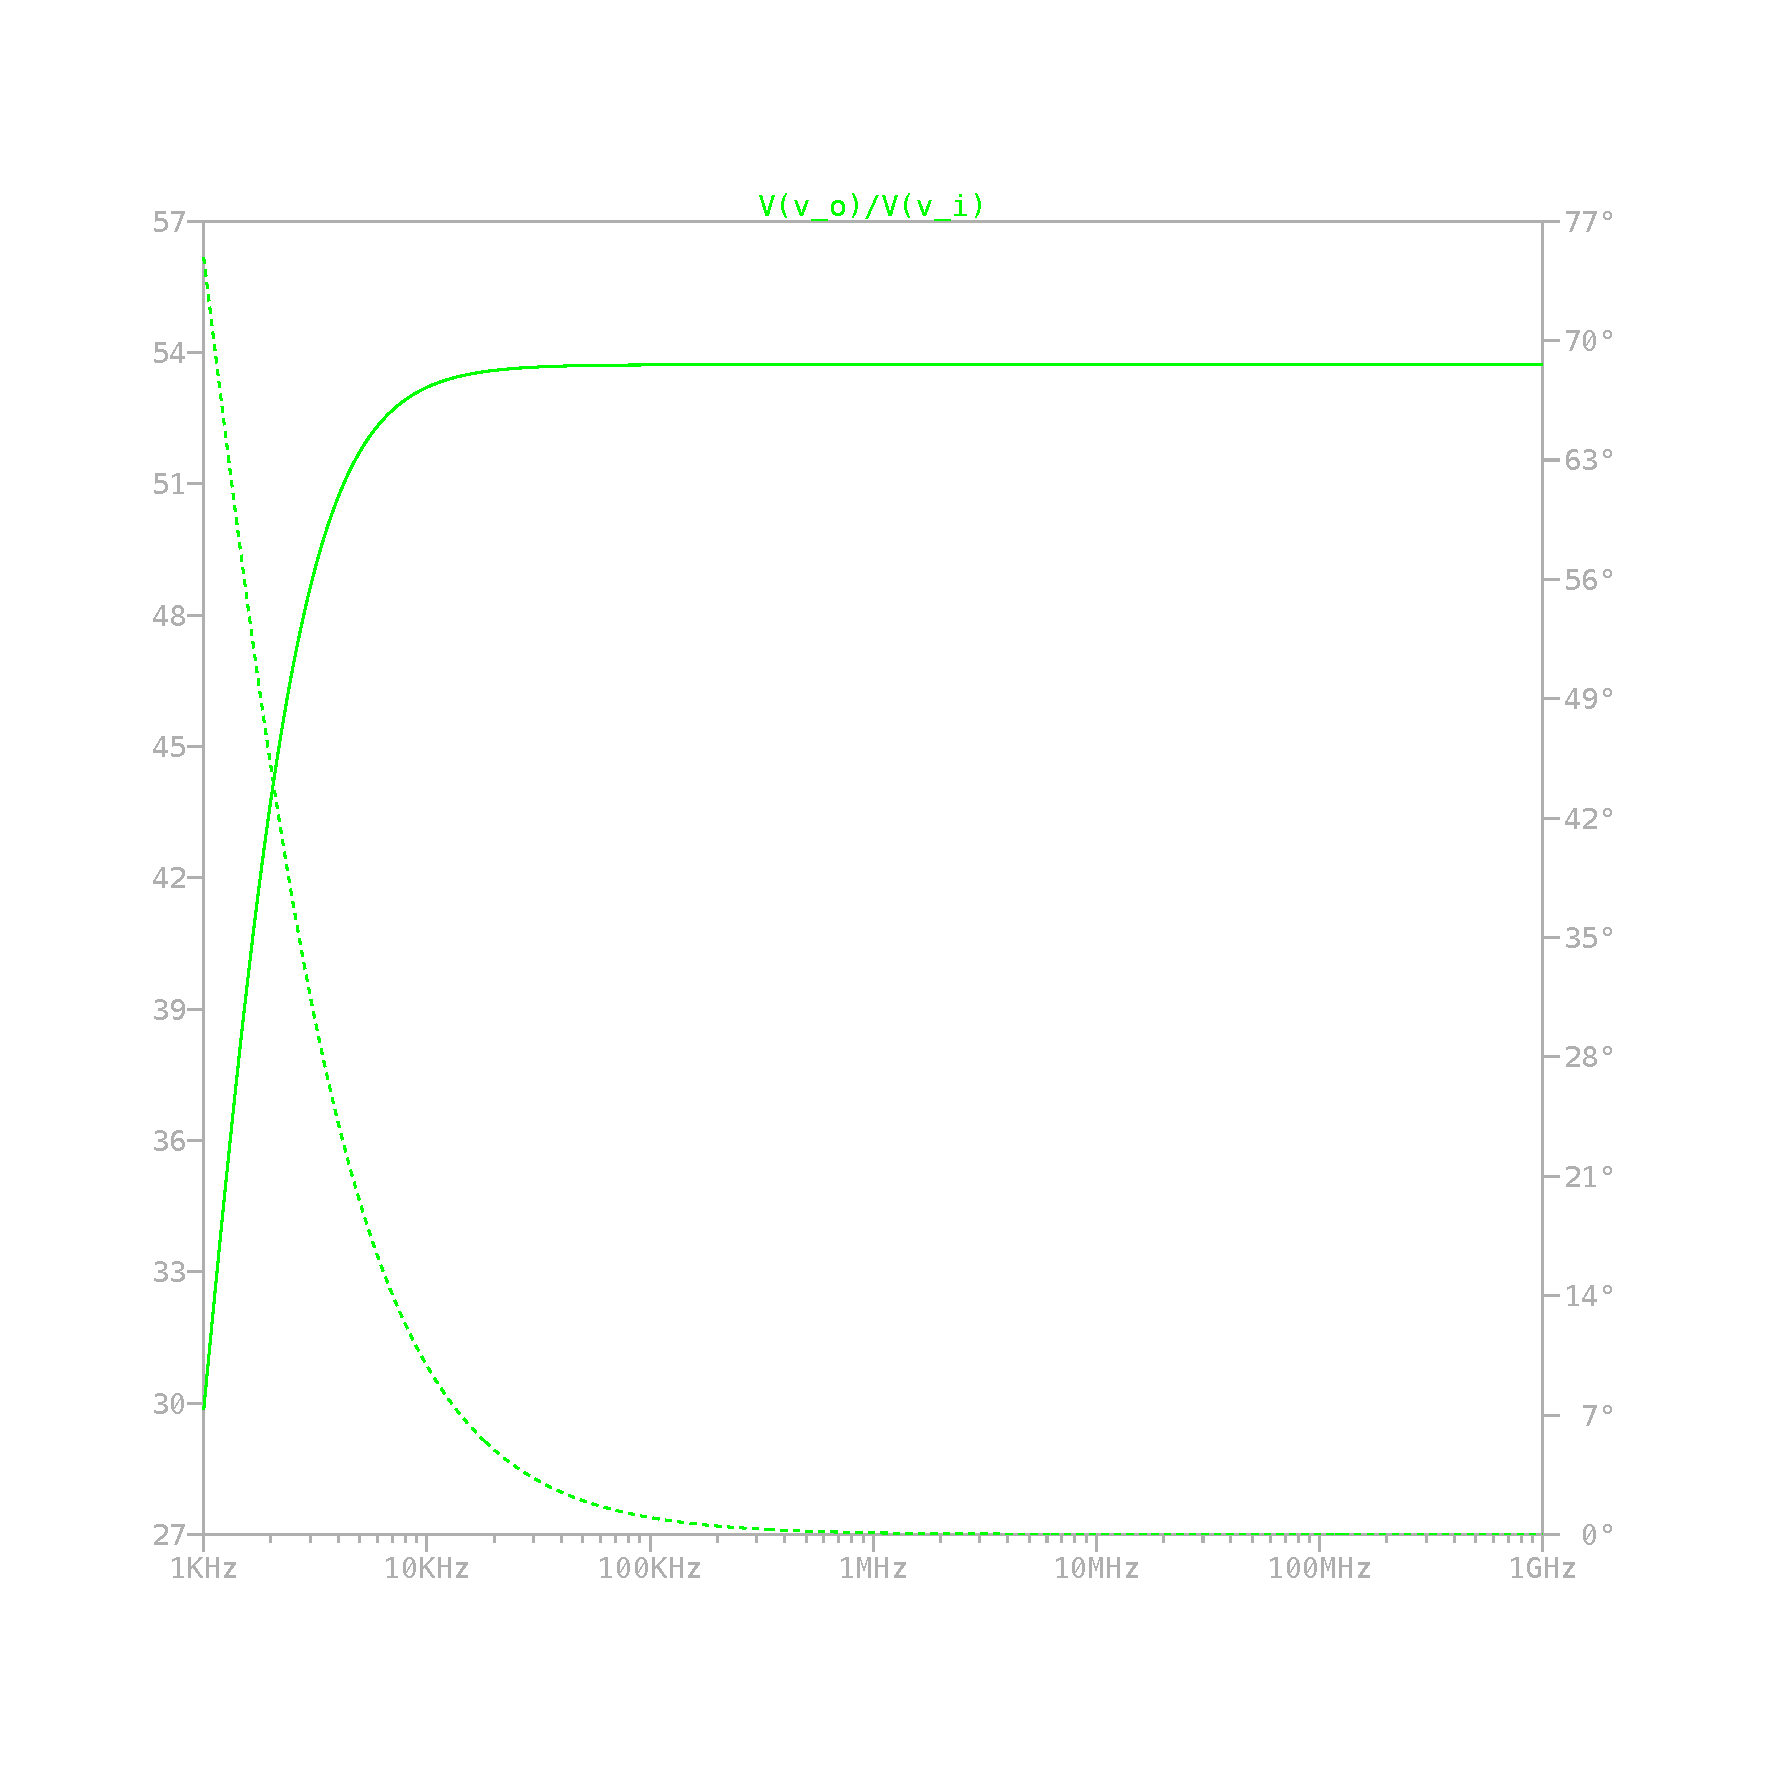
\includegraphics[height=0.4\textheight,trim={30mm 30mm 30mm 30mm}]{img/Amplifier Design Gain.pdf}
    \caption{Gain of the Amplifier Circuit}
    \label{fig:ac-gain}
\end{figure}

\begin{figure}[H]
    \centering
    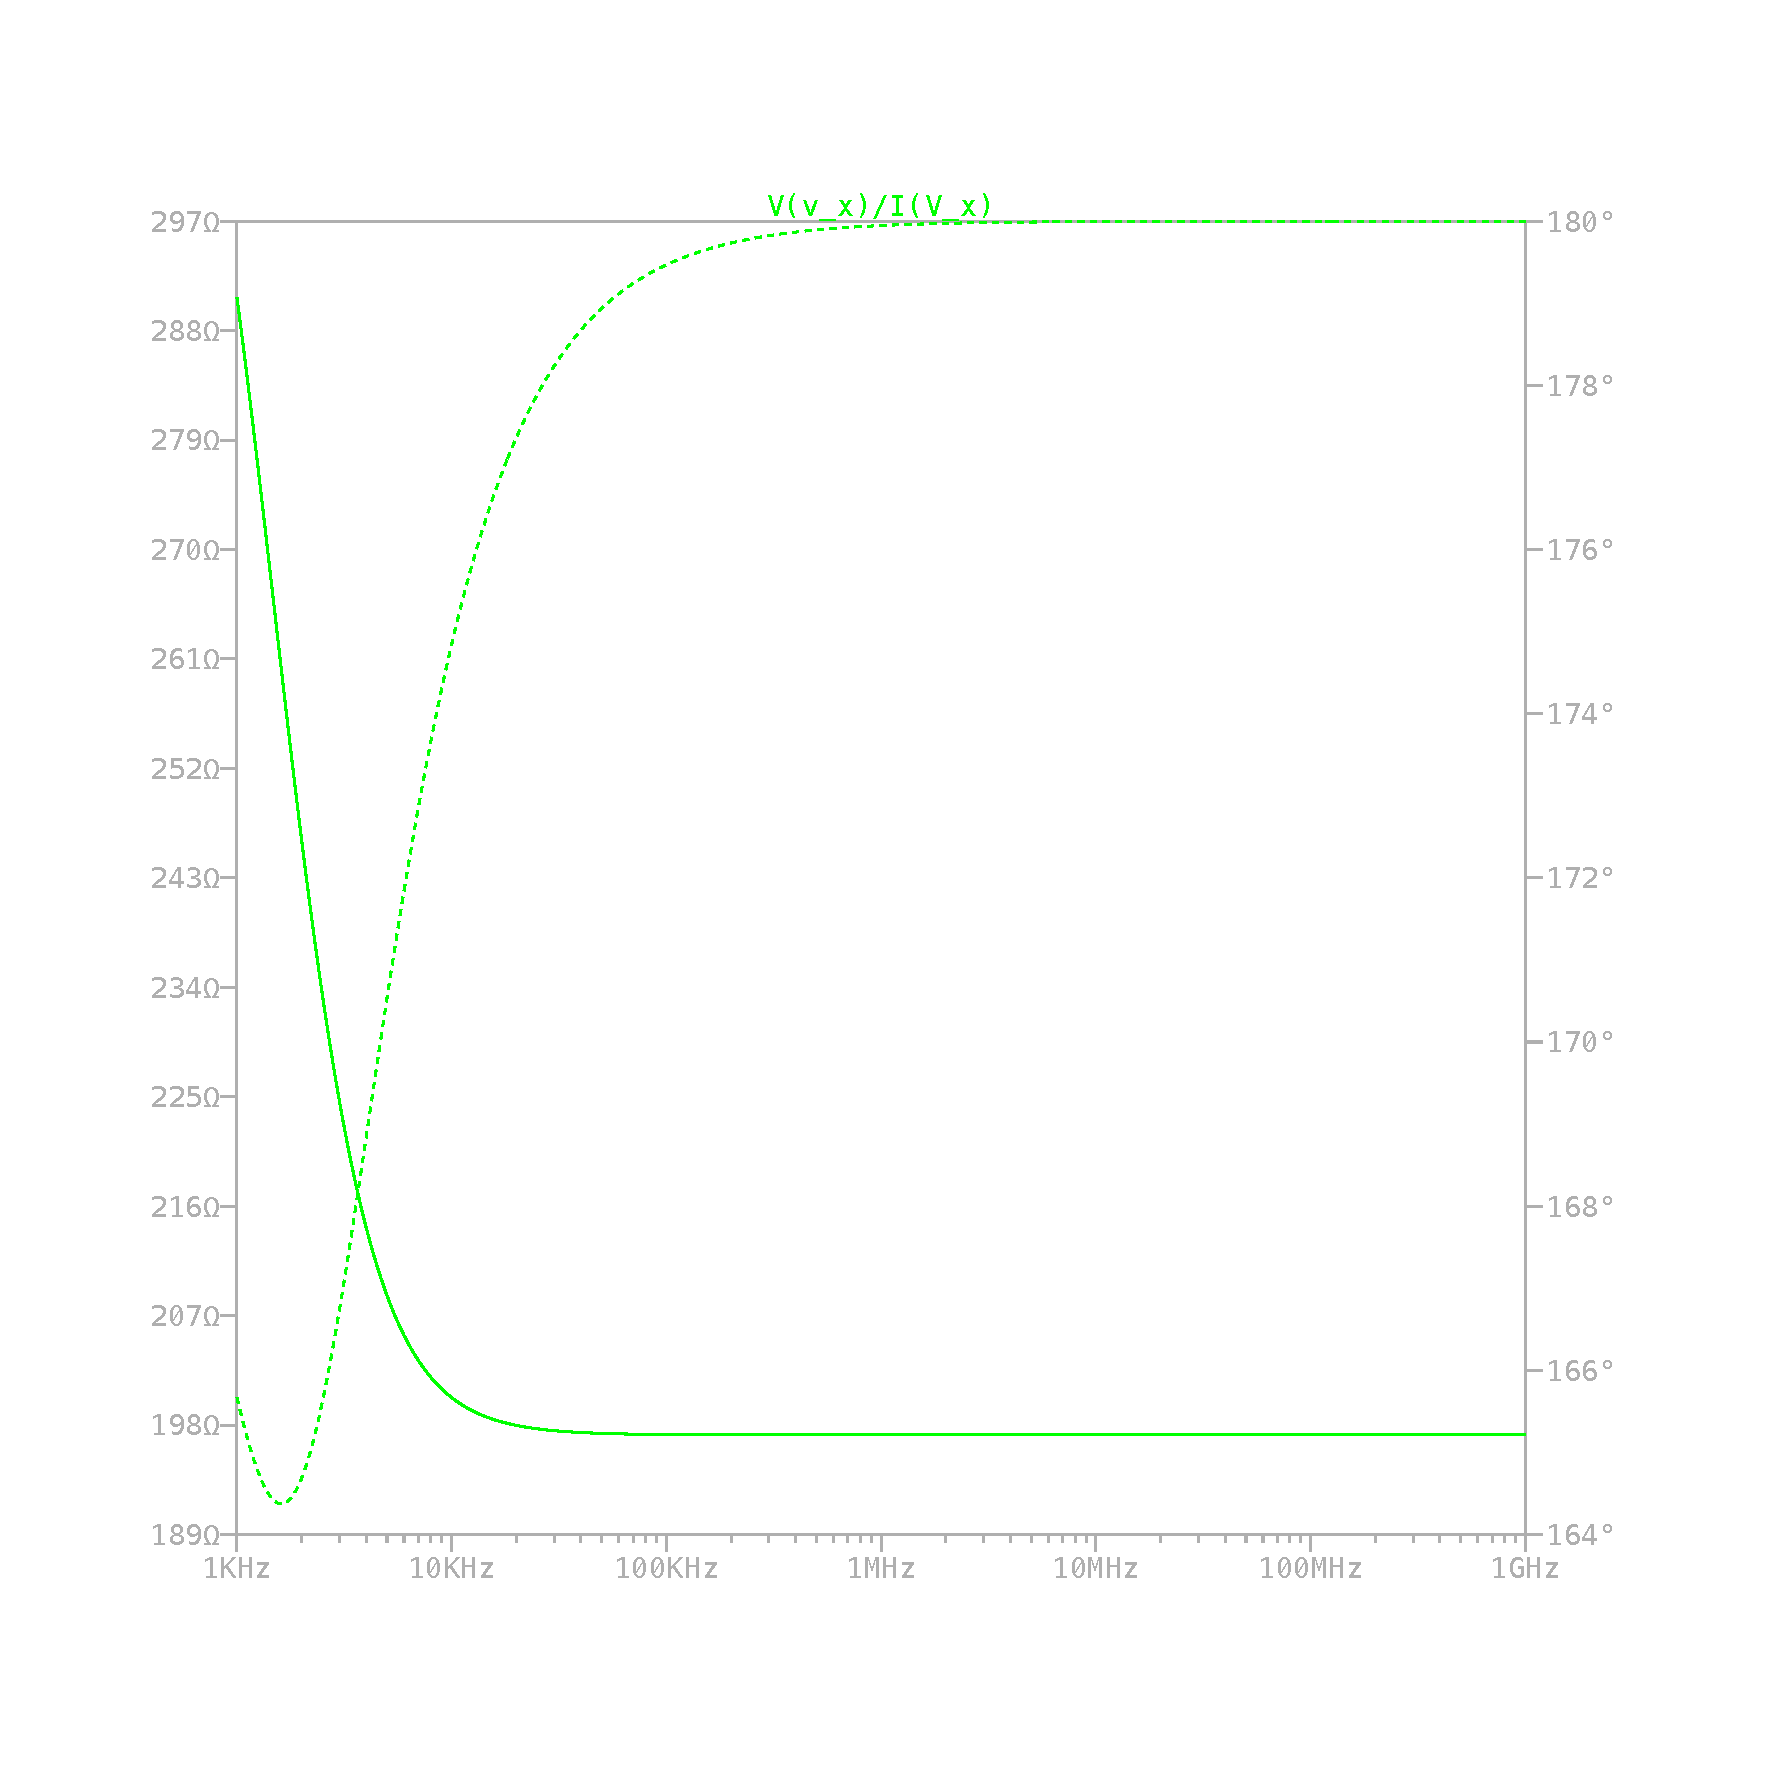
\includegraphics[height=0.4\textheight,trim={30mm 30mm 30mm 30mm}]{img/Amplifier Design Input Resistance.pdf}
    \caption{Input Resistance of the Amplifier Circuit}
    \label{fig:ac-input-res}
\end{figure}

\begin{figure}[H]
    \centering
    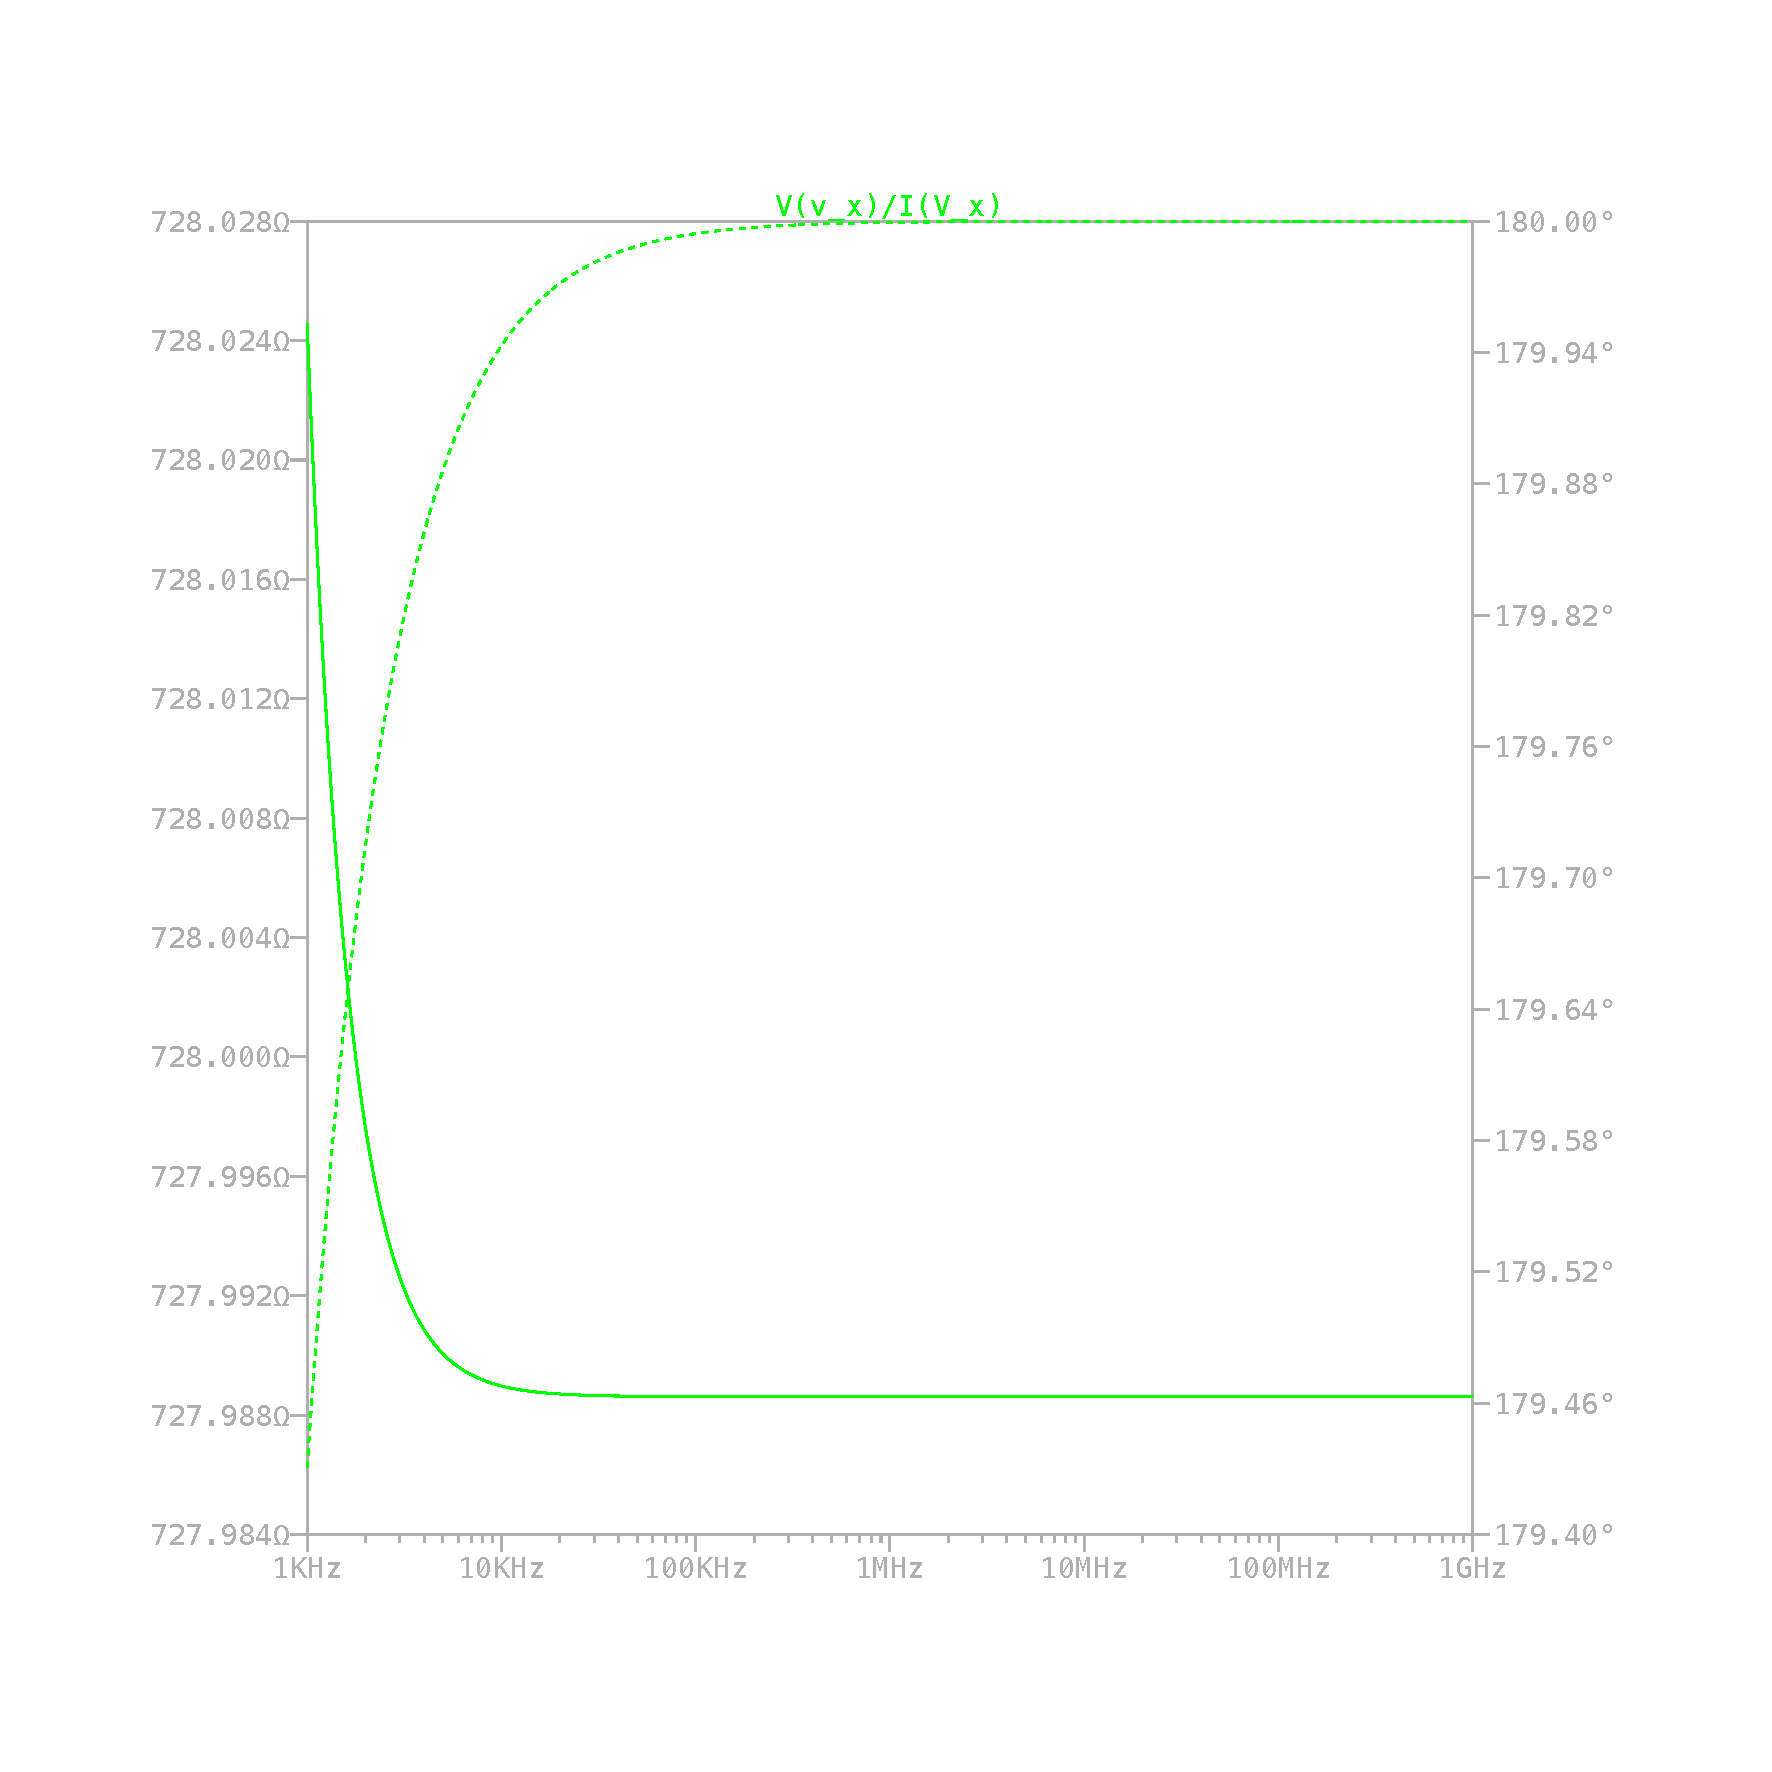
\includegraphics[height=0.4\textheight,trim={30mm 30mm 30mm 30mm}]{img/Amplifier Design Output Resistance.pdf}
    \caption{Output Resistance of the Amplifier Circuit}
    \label{fig:ac-output-res}
\end{figure}

\section{Circuit Modification}

A new design requirement is imposed to explore other possibility of the amplifier design.
A gain of smaller than the calculated gain with \ang{0} phase shift is imposed as the new design requirements.
This new design requirements must be achieved without changing the transistor, designed voltage and resistors (including changing, removing or adding).

In order to meet a new design requirements, the transistor configurations of the BJT amplifier is modified into common collectors.
As a result of changing the configuration, the bypass capacitors are removed at the emitter.
This is because the bypass capacitor will short the voltage to the next stage to ground resulting in 0 gain no matter what.
Figure \ref{fig:new-amp-circuit} shows the new amplifier circuit.

Upon changing the BJT configuration to common collector, the voltage gain of the amplifier is reduced.
This is due to one of the assumption made which is the gain of a common collector amplifier is around 1 and the gain of a common emitter amplifier is grater than 1.
The general formula for the gain of a cascaded amplifier is the gain of all the transistor multiplied together, therefore changing the BJT amplifier to common collector decreases the overall gain.
Furthermore, the DC analysis is assumed to be the same, as the resistor location and values remained the same.
Lastly, changing a BJT amplifier to common collector will bring a \ang{180} phase shift to the gain.
Therefore, both the BJT amplifier are changed in the circuit into a common collector to bring the phase shift back to \ang{0}.

\begin{figure}[H]
    \centering
    \resizebox{\textwidth}{!}{
        \begin{circuitikz}[american]
            % Input Voltage
            \draw (0, 0) to[resistor, R=$R_{S}$] (2, 0) to[capacitor, -*] (4, 0);
            \draw (0, 0) to [vsource, V=$V_{s}$] (0, -3) to (4, -3);

            % Q1
            \draw (6, 0) node[npn](Q1){Q1};
            \draw (4, 0) to (Q1.B);
            \draw (Q1.E) to[resistor, R=$R_{E1}$, -*] (6, -3) to ++(-5, 0);
            \draw (6, 3) to[resistor, R=$R_{C1}$] (Q1.C);
            \draw (6, 3) to[short, *-] (4, 3) to[resistor, R=$R_{11}$] (4, 0) to[resistor, R=$R_{21}$, -*] (4, -3);
            % Coupling Capacitor
            \draw (Q1.E) to[capacitor] ++(2, 0) to (8, 0) to[short, -*] ++(1, 0);

            % Q2
            \draw (11, 0) node[npn](Q2){Q2};
            \draw (9, 0) to (Q2.B);
            \draw (Q2.E) to[resistor, R=$R_{E2}$, -*] (11, -3) to ++(-5, 0);
            \draw (11, 3) to[resistor, R=$R_{C2}$] (Q2.C);
            \draw (6, 3) to[short, -*] (9, 3) to[resistor, R=$R_{12}$] ++(0, -3) to[resistor, R=$R_{22}$, -*] ++(0, -3);
            \draw (9, 3) to[short, -*] ++(2, 0);
            % Coupling Capacitor
            \draw (Q2.E) to[capacitor] ++(2, 0) to (13, 0) to[short, -*] ++(1, 0) node[anchor=east](M3_start){};

            % M3
            \draw (M3_start) ++(2, 0) node[nmos](M3){M3};
            \draw (M3_start) to (M3.G);
            \draw (11, 3) to[short, -*] ++(3, 0) to[resistor, R=$R_{13}$] ++(0, -3) to[resistor, R=$R_{23}$, -*] ++(0, -3) to ++(-3, 0);
            \draw (M3.D) to[short, -o] ++(0, 2.23) node[anchor=west]{$V_{CC}$} to ++(-2, 0);
            % https://tex.stackexchange.com/questions/18389/tikz-node-at-same-x-coordinate-as-another-node-but-specified-y-coordinate
            \draw (M3.S) to[resistor, R=$R_{SS}$, *-*] (M3.S |-, -3) to ++(2, 0) node[anchor=north](R_L){};
            \draw (M3.S) to[capacitor] ++(2, 0) to[resistor, R=$R_{L}$] (R_L);
            \draw (M3.S |-, -3) to ++(-2, 0);

            % Vo
            \draw (M3.S) ++(2, 0) to[short, -o] ++(0.5, 0) node[anchor=west]{$v_o$};
            % Ground
            \draw (Q2.E |-, -3) to (Q2.E |-, -3.1) node[ground]{};
        \end{circuitikz}
    }
    \caption{New Amplifier Circuit}
    \label{fig:new-amp-circuit}
\end{figure}

\clearpage{}

\printbibliography{}

\clearpage{}

\section{Appendix}

These are the LTSpice circuit used.
They are ordered shown below:
\begin{enumerate}
    \item DC Analysis
    \item AC Gain Analysis
    \item AC Input Resistance Analysis
    \item AC Output Resistance Analysis
\end{enumerate}

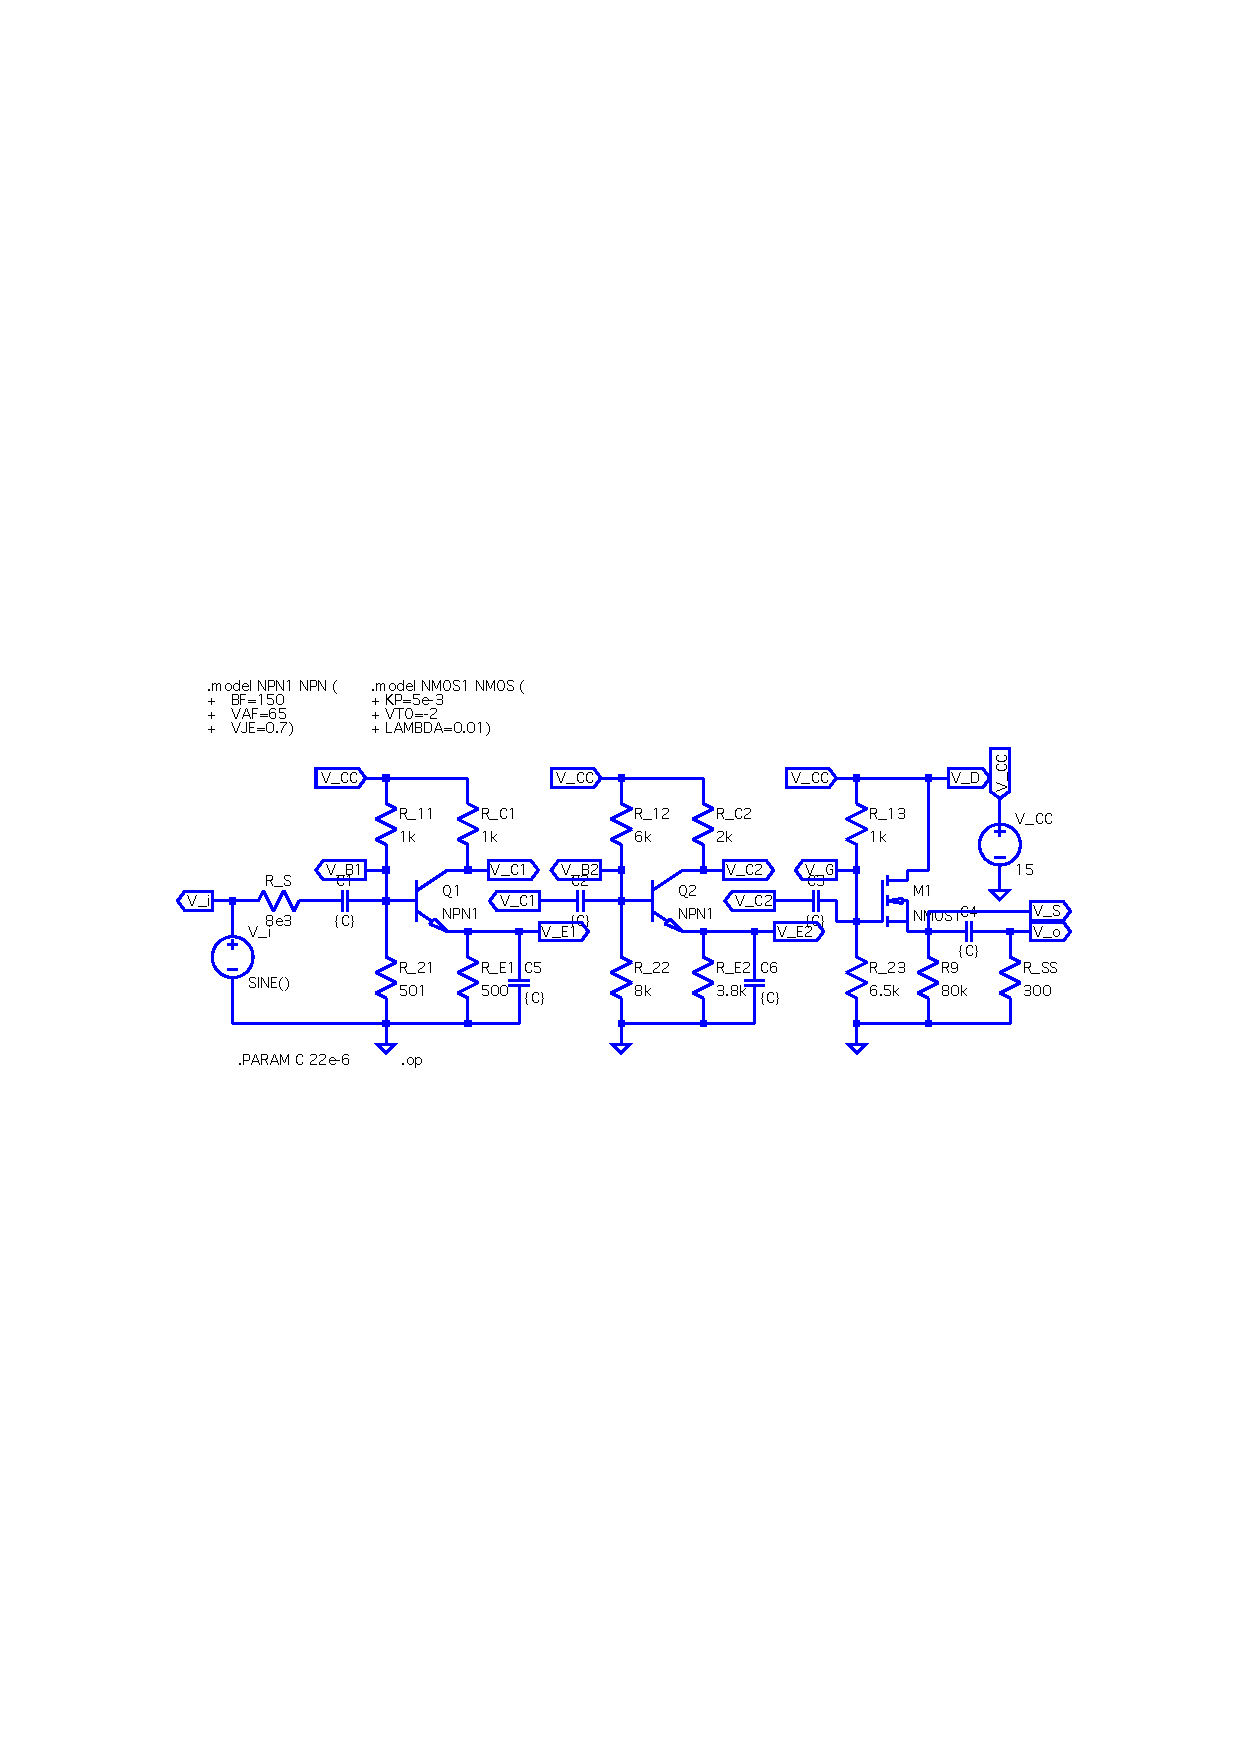
\includepdf{img/DC Circuit.pdf}
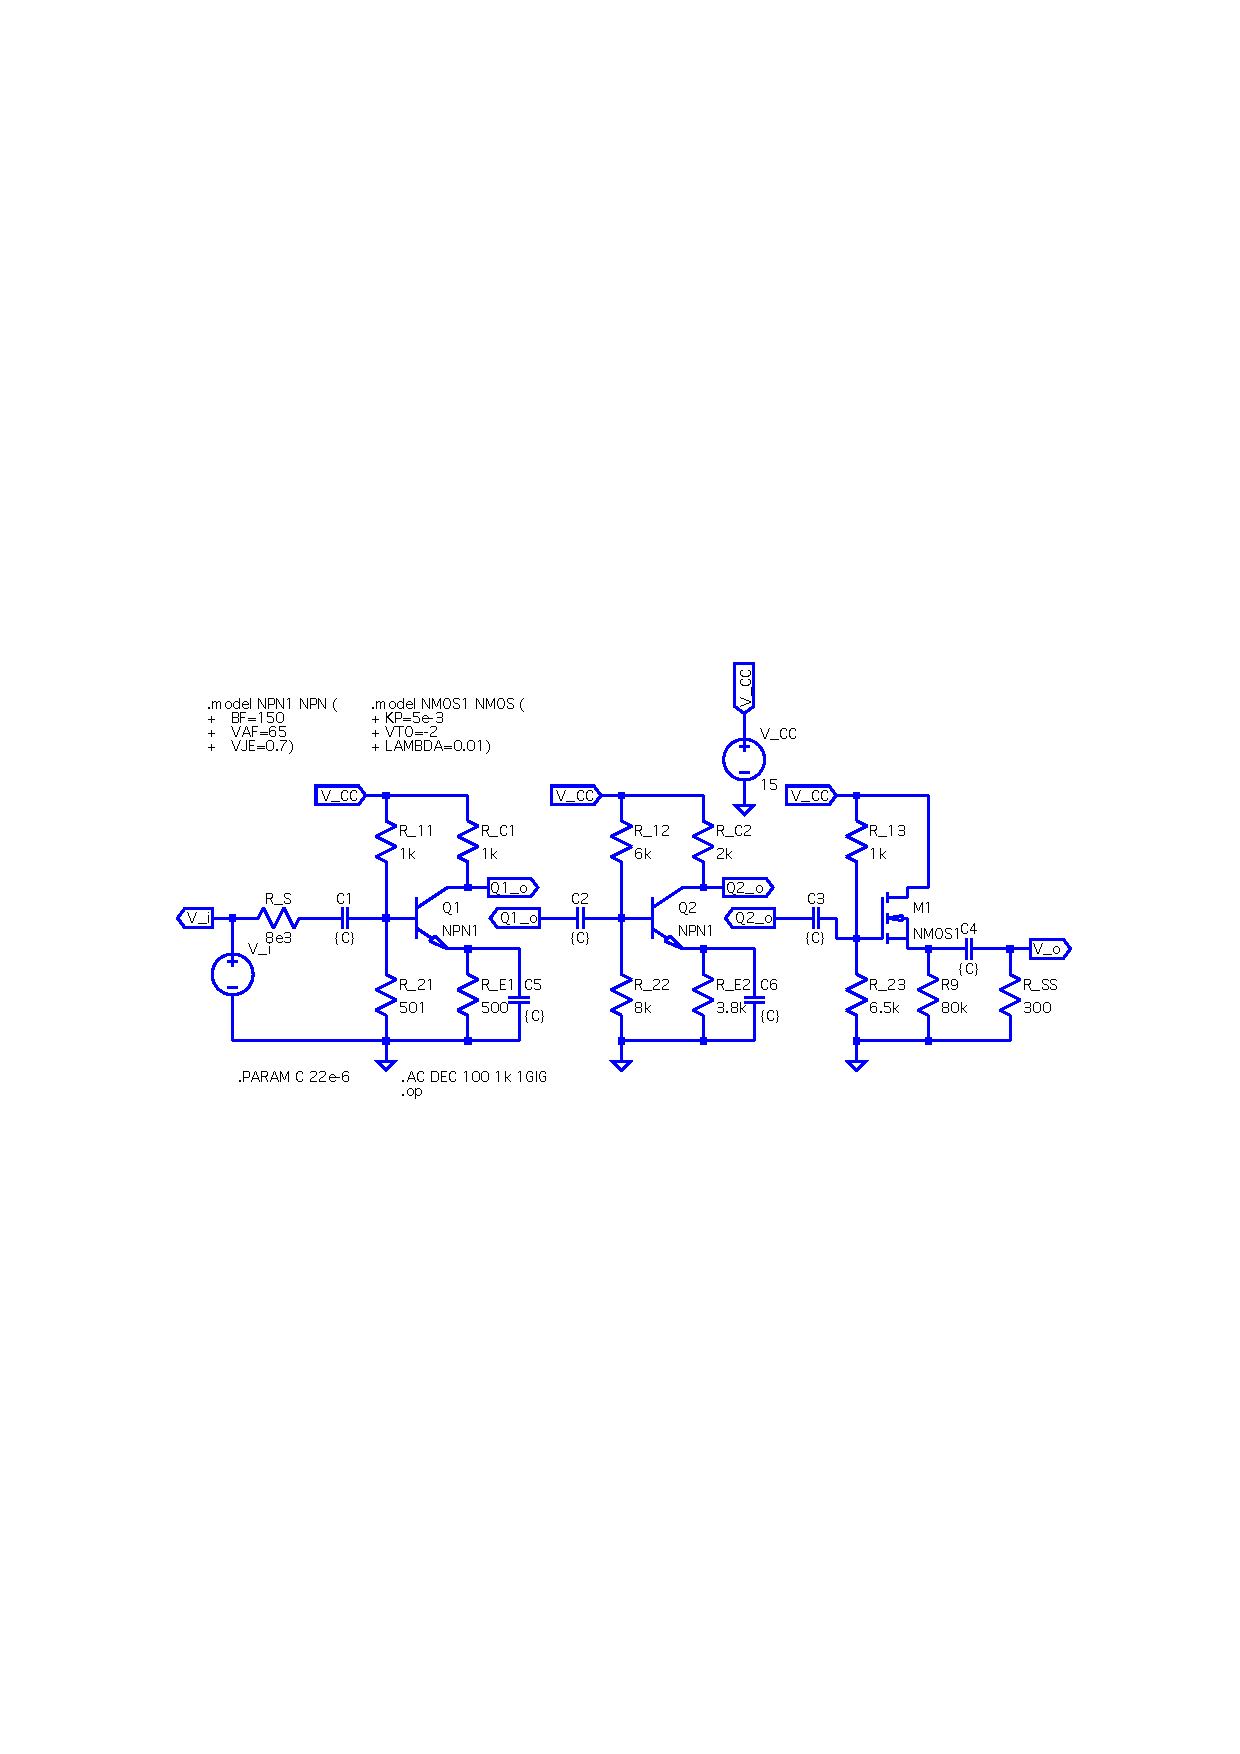
\includepdf{img/Gain Circuit.pdf}
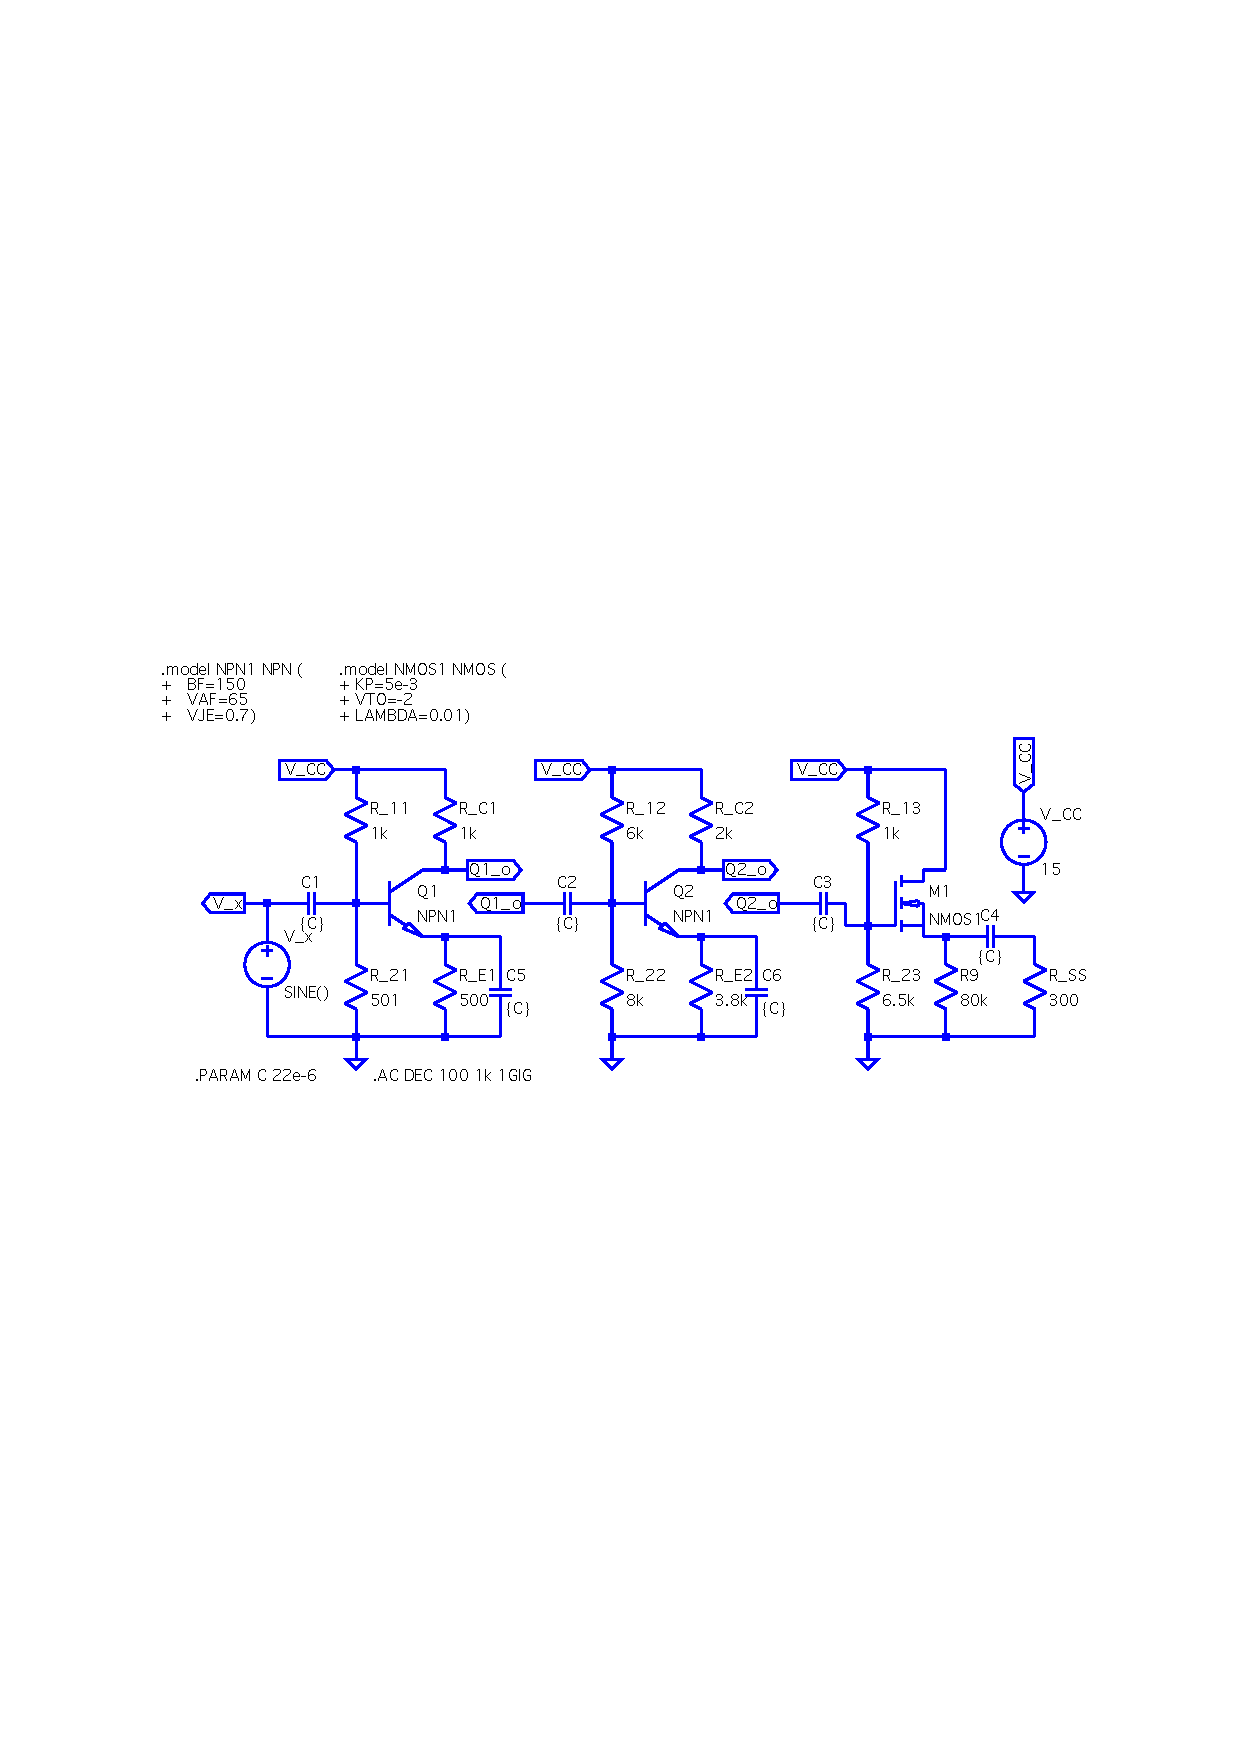
\includepdf{img/Input Resistance Circuit.pdf}
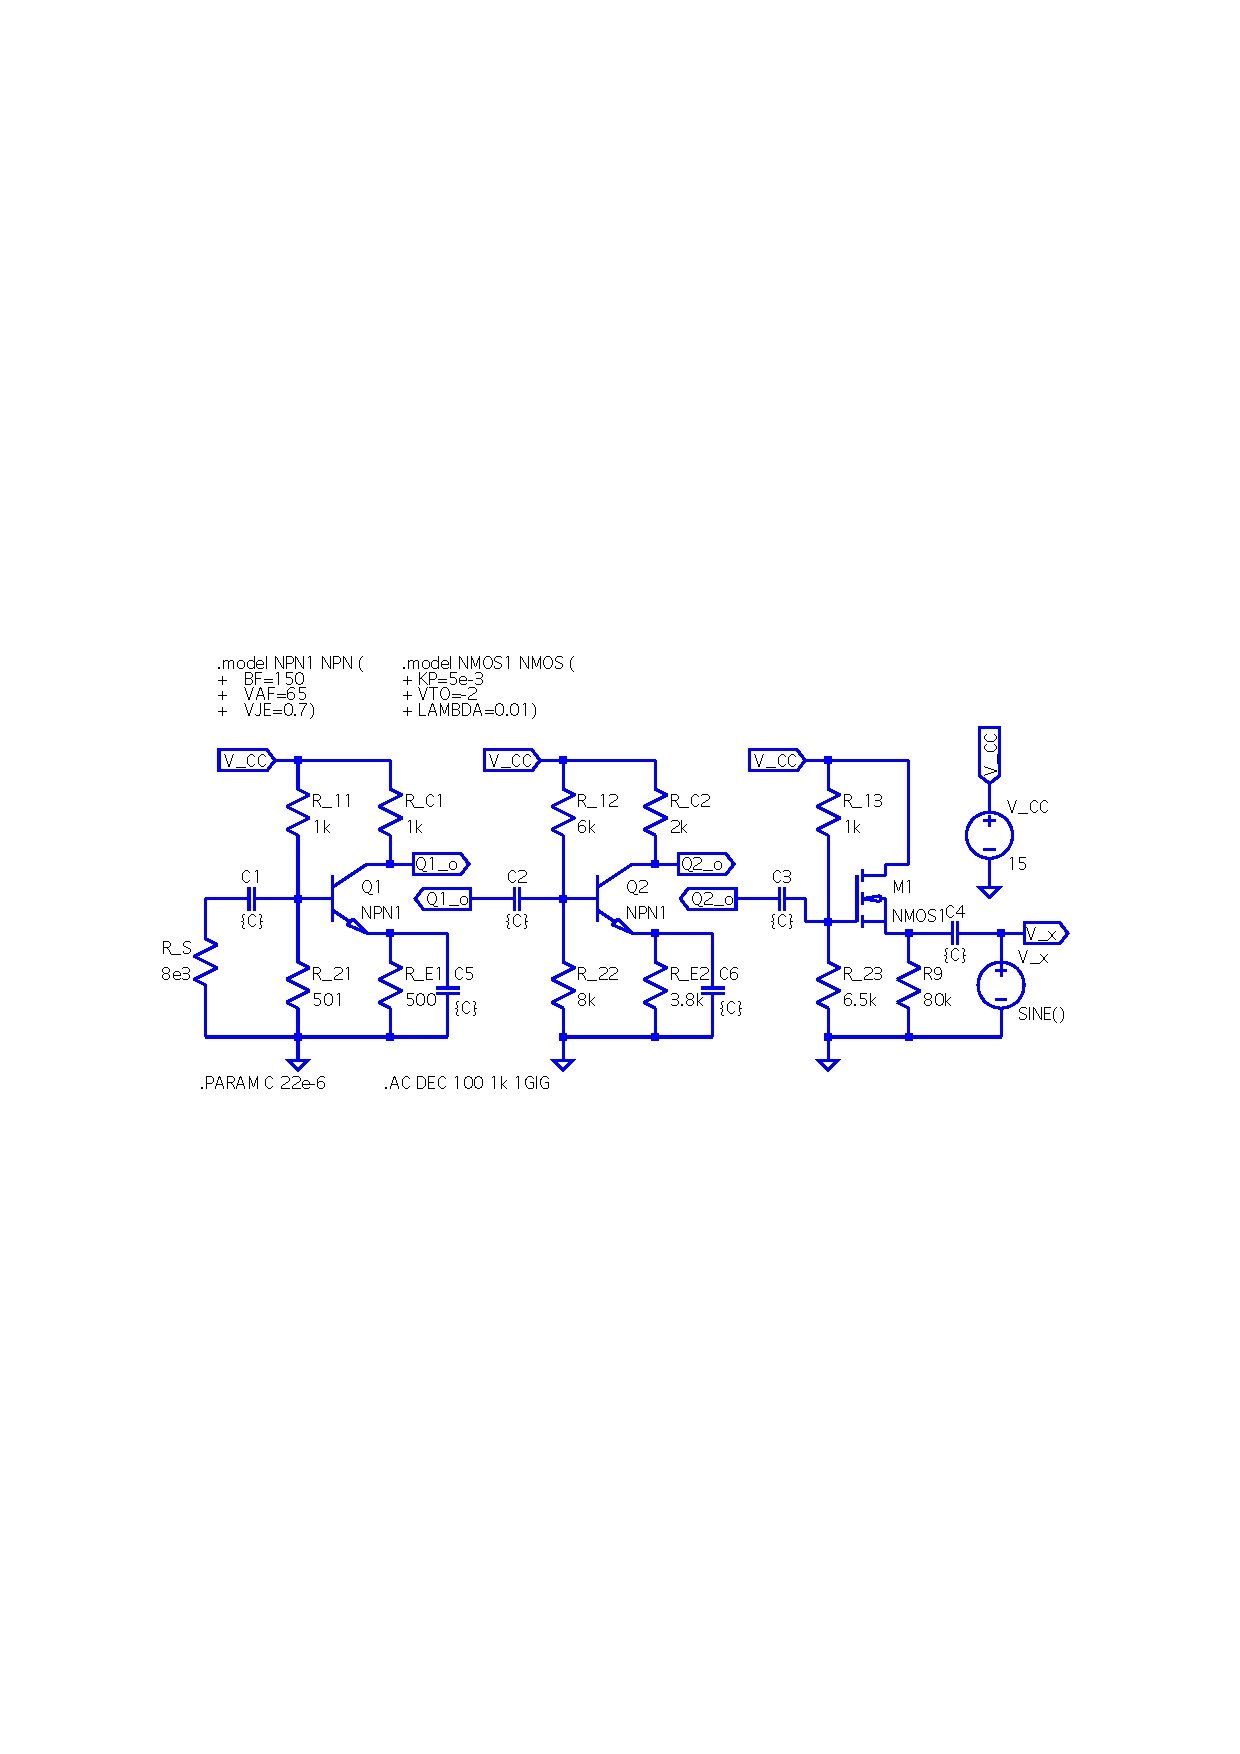
\includepdf{img/Output Resistance Circuit.pdf}

\end{document}
